\documentclass[preprint,12pt]{elsarticle}
\usepackage{amsmath,amssymb,amsthm}
\usepackage{graphicx}
\usepackage{booktabs}
\usepackage{url}
\usepackage{algorithm,algpseudocode}
\journal{Neurocomputing}
% Contract v4 measured-value macros (regenerated from real results;
% this file is rewritten from scratch on every fill run).
\newcommand{\AgreeCfivemtEnron}{1.0000}
\newcommand{\AgreeCfivemtLastfm}{0.9986}
\newcommand{\AgreeCfivemtMooc}{1.0000}
\newcommand{\AgreeCfivemtReddit}{1.0000}
\newcommand{\AgreeCfivemtWikipedia}{0.9994}
\newcommand{\AgreeEnron}{1.0000}
\newcommand{\AgreeLastfm}{0.9995}
\newcommand{\AgreeMooc}{1.0000}
\newcommand{\AgreeReddit}{1.0000}
\newcommand{\AgreeSdEnron}{0.00014}
\newcommand{\AgreeSdLastfm}{0.00151}
\newcommand{\AgreeSdMooc}{0.00000}
\newcommand{\AgreeSdReddit}{0.00000}
\newcommand{\AgreeSdWikipedia}{0.00041}
\newcommand{\AgreeTeightCtwo}{1.0000}
\newcommand{\AgreeTeightMzero}{1.0000}
\newcommand{\AgreeTfourCtwo}{1.0000}
\newcommand{\AgreeTfourMzero}{1.0000}
\newcommand{\AgreeToneCtwo}{1.0000}
\newcommand{\AgreeToneMzero}{1.0000}
\newcommand{\AgreeTsixteenCtwo}{1.0000}
\newcommand{\AgreeTsixteenMzero}{1.0000}
\newcommand{\AgreeTtwoCtwo}{1.0000}
\newcommand{\AgreeTtwoMzero}{1.0000}
\newcommand{\AgreeWikipedia}{0.9997}
\newcommand{\AllFiveConjunction}{false}
\newcommand{\AnnRefEnron}{7065.600}
\newcommand{\AnnRefLastfm}{7065.600}
\newcommand{\AnnRefMooc}{7065.600}
\newcommand{\AnnRefReddit}{7065.600}
\newcommand{\AnnRefWikipedia}{7065.600}
\newcommand{\BHqEnron}{0.2376}
\newcommand{\BHqLastfm}{0.4453}
\newcommand{\BHqMooc}{0.4453}
\newcommand{\BHqReddit}{0.2376}
\newcommand{\BHqWikipedia}{0.03906}
\newcommand{\BoundRtwoEnron}{0.908}
\newcommand{\BoundRtwoLastfm}{0.921}
\newcommand{\BoundRtwoMooc}{0.896}
\newcommand{\BoundRtwoReddit}{0.874}
\newcommand{\BoundRtwoWikipedia}{0.922}
\newcommand{\CHatEnron}{0.000}
\newcommand{\CHatLastfm}{0.000}
\newcommand{\CHatMooc}{0.000}
\newcommand{\CHatReddit}{0.000}
\newcommand{\CHatWikipedia}{0.000}
\newcommand{\CIDiffEnronHi}{0.00075}
\newcommand{\CIDiffEnronLo}{-0.00018}
\newcommand{\CIDiffLastfmHi}{0.00018}
\newcommand{\CIDiffLastfmLo}{-0.00006}
\newcommand{\CIDiffMoocHi}{0.00007}
\newcommand{\CIDiffMoocLo}{-0.00017}
\newcommand{\CIDiffRedditHi}{0.00020}
\newcommand{\CIDiffRedditLo}{-0.00002}
\newcommand{\CIDiffWikipediaHi}{0.00075}
\newcommand{\CIDiffWikipediaLo}{0.00028}
\newcommand{\DReplicationTenSeed}{false}
\newcommand{\DownSlopeEnron}{-0.00000}
\newcommand{\DownSlopeLastfm}{-0.00000}
\newcommand{\DownSlopeMooc}{0.00000}
\newcommand{\DownSlopeReddit}{-0.00000}
\newcommand{\DownSlopeWikipedia}{-0.00000}
\newcommand{\DriftRelEnron}{0.0576}
\newcommand{\DriftRelLastfm}{0.1224}
\newcommand{\DriftRelMooc}{0.0628}
\newcommand{\DriftRelReddit}{0.1382}
\newcommand{\DriftRelWikipedia}{0.1875}
\newcommand{\DzEnron}{0.53}
\newcommand{\DzLastfm}{0.27}
\newcommand{\DzMooc}{-0.25}
\newcommand{\DzReddit}{0.50}
\newcommand{\DzWikipedia}{1.27}
\newcommand{\EnergyCfivemtEnron}{16.361}
\newcommand{\EnergyCfivemtLastfm}{16.254}
\newcommand{\EnergyCfivemtMooc}{17.249}
\newcommand{\EnergyCfivemtReddit}{15.687}
\newcommand{\EnergyCfivemtWikipedia}{16.661}
\newcommand{\EnergyCtwoEnron}{110.189}
\newcommand{\EnergyCtwoLastfm}{97.359}
\newcommand{\EnergyCtwoMooc}{105.903}
\newcommand{\EnergyCtwoReddit}{101.819}
\newcommand{\EnergyCtwoWikipedia}{102.928}
\newcommand{\EnergyMzeroEnron}{114.062}
\newcommand{\EnergyMzeroLastfm}{99.501}
\newcommand{\EnergyMzeroMooc}{106.731}
\newcommand{\EnergyMzeroReddit}{102.785}
\newcommand{\EnergyMzeroWikipedia}{104.443}
\newcommand{\EnergyRatioCfivemtEnron}{0.0023}
\newcommand{\EnergyRatioCfivemtLastfm}{0.0023}
\newcommand{\EnergyRatioCfivemtMooc}{0.0024}
\newcommand{\EnergyRatioCfivemtReddit}{0.0022}
\newcommand{\EnergyRatioCfivemtWikipedia}{0.0024}
\newcommand{\EnergyRatioCtwoEnron}{0.0156}
\newcommand{\EnergyRatioCtwoLastfm}{0.0138}
\newcommand{\EnergyRatioCtwoMooc}{0.0150}
\newcommand{\EnergyRatioCtwoReddit}{0.0144}
\newcommand{\EnergyRatioCtwoWikipedia}{0.0146}
\newcommand{\EnergyRatioMzeroEnron}{0.0161}
\newcommand{\EnergyRatioMzeroLastfm}{0.0141}
\newcommand{\EnergyRatioMzeroMooc}{0.0151}
\newcommand{\EnergyRatioMzeroReddit}{0.0145}
\newcommand{\EnergyRatioMzeroWikipedia}{0.0148}
\newcommand{\EpsCfivemtEnron}{0.00660}
\newcommand{\EpsCfivemtLastfm}{0.00662}
\newcommand{\EpsCfivemtMooc}{0.00529}
\newcommand{\EpsCfivemtReddit}{0.00623}
\newcommand{\EpsCfivemtWikipedia}{0.00679}
\newcommand{\EpsCtwoEnron}{0.00553}
\newcommand{\EpsCtwoLastfm}{0.00424}
\newcommand{\EpsCtwoMooc}{0.00368}
\newcommand{\EpsCtwoReddit}{0.00361}
\newcommand{\EpsCtwoWikipedia}{0.00514}
\newcommand{\EpsMzeroEnron}{0.00514}
\newcommand{\EpsMzeroLastfm}{0.00418}
\newcommand{\EpsMzeroMooc}{0.00373}
\newcommand{\EpsMzeroReddit}{0.00351}
\newcommand{\EpsMzeroWikipedia}{0.00465}
\newcommand{\EtaEnron}{0.003}
\newcommand{\EtaLastfm}{0.003}
\newcommand{\EtaMooc}{0.004}
\newcommand{\EtaReddit}{0.005}
\newcommand{\EtaWikipedia}{0.004}
\newcommand{\EvCfivemtEnron}{6.060}
\newcommand{\EvCfivemtLastfm}{6.020}
\newcommand{\EvCfivemtMooc}{6.389}
\newcommand{\EvCfivemtReddit}{5.810}
\newcommand{\EvCfivemtWikipedia}{6.171}
\newcommand{\EvCtwoEnron}{40.811}
\newcommand{\EvCtwoLastfm}{36.059}
\newcommand{\EvCtwoMooc}{39.223}
\newcommand{\EvCtwoReddit}{37.711}
\newcommand{\EvCtwoWikipedia}{38.121}
\newcommand{\EvMzeroEnron}{42.245}
\newcommand{\EvMzeroLastfm}{36.852}
\newcommand{\EvMzeroMooc}{39.530}
\newcommand{\EvMzeroReddit}{38.068}
\newcommand{\EvMzeroWikipedia}{38.683}
\newcommand{\FiringMzeroEnron}{0.66008}
\newcommand{\FiringMzeroLastfm}{0.57582}
\newcommand{\FiringMzeroMooc}{0.61766}
\newcommand{\FiringMzeroReddit}{0.59482}
\newcommand{\FiringMzeroWikipedia}{0.60441}
\newcommand{\IndGapCfivemtEnron}{0.00}
\newcommand{\IndGapCfivemtMooc}{0.00}
\newcommand{\IndGapCfivemtReddit}{0.00}
\newcommand{\IndGapCfivemtWikipedia}{0.06}
\newcommand{\IndGapCtwoEnron}{0.00}
\newcommand{\IndGapCtwoMooc}{0.00}
\newcommand{\IndGapCtwoReddit}{0.00}
\newcommand{\IndGapCtwoWikipedia}{0.03}
\newcommand{\IndGapMzeroEnron}{0.00}
\newcommand{\IndGapMzeroMooc}{0.00}
\newcommand{\IndGapMzeroReddit}{0.00}
\newcommand{\IndGapMzeroWikipedia}{0.03}
\newcommand{\LAEnron}{0.016}
\newcommand{\LALastfm}{0.007}
\newcommand{\LAMooc}{0.012}
\newcommand{\LAReddit}{0.008}
\newcommand{\LAWikipedia}{0.039}
\newcommand{\LatencyAFive}{0.250}
\newcommand{\LatencyAOne}{0.305}
\newcommand{\LatencyAThree}{0.266}
\newcommand{\LatencyATwo}{0.265}
\newcommand{\LatencyCOne}{0.252}
\newcommand{\LatencyCfivemt}{0.090}
\newcommand{\LatencyCfour}{0.106}
\newcommand{\LatencyCthree}{0.096}
\newcommand{\LatencyCtwo}{0.277}
\newcommand{\LatencyCzero}{0.105}
\newcommand{\LatencyDOne}{0.081}
\newcommand{\LatencyMzero}{0.257}
\newcommand{\MeanDeltaA}{0.319}
\newcommand{\MeanDiffEnron}{3.96e-04}
\newcommand{\MeanDiffLastfm}{5.57e-05}
\newcommand{\MeanDiffMooc}{-5.05e-05}
\newcommand{\MeanDiffReddit}{9.59e-05}
\newcommand{\MeanDiffWikipedia}{4.90e-04}
\newcommand{\NMethods}{12}
\newcommand{\NRefs}{50}
\newcommand{\NRuns}{50}
\newcommand{\NSeeds}{10}
\newcommand{\OverheadCfivemtEnron}{-85.15}
\newcommand{\OverheadCfivemtLastfm}{-83.30}
\newcommand{\OverheadCfivemtMooc}{-83.71}
\newcommand{\OverheadCfivemtReddit}{-84.59}
\newcommand{\OverheadCfivemtWikipedia}{-83.81}
\newcommand{\OverheadTcarEnron}{1.710}
\newcommand{\OverheadTcarLastfm}{1.607}
\newcommand{\OverheadTcarMooc}{1.202}
\newcommand{\OverheadTcarReddit}{2.108}
\newcommand{\OverheadTcarWikipedia}{2.748}
\newcommand{\PoIEnron}{0.052}
\newcommand{\PoILastfm}{0.182}
\newcommand{\PoIMooc}{0.797}
\newcommand{\PoIReddit}{0.050}
\newcommand{\PoIWikipedia}{0.000}
\newcommand{\RedEnron}{7.2\%}
\newcommand{\RedLastfm}{1.3\%}
\newcommand{\RedMooc}{-1.4\%}
\newcommand{\RedReddit}{2.7\%}
\newcommand{\RedWikipedia}{9.5\%}
\newcommand{\RetEnron}{1.0001}
\newcommand{\RetLastfm}{1.0000}
\newcommand{\RetMooc}{1.0000}
\newcommand{\RetReddit}{1.0000}
\newcommand{\RetWikipedia}{1.0003}
\newcommand{\RhoEnron}{0.784}
\newcommand{\RhoLastfm}{0.677}
\newcommand{\RhoMooc}{0.668}
\newcommand{\RhoReddit}{0.722}
\newcommand{\RhoWikipedia}{0.727}
\newcommand{\RobustCleanDropCtwo}{5.05e-03}
\newcommand{\RobustCleanDropMzero}{4.27e-03}
\newcommand{\RobustCleanDtCtwo}{5.05e-03}
\newcommand{\RobustCleanDtMzero}{4.27e-03}
\newcommand{\RobustCleanNoiseCtwo}{5.05e-03}
\newcommand{\RobustCleanNoiseMzero}{4.27e-03}
\newcommand{\RobustMaxDropCtwo}{5.05e-03}
\newcommand{\RobustMaxDropMzero}{4.27e-03}
\newcommand{\RobustMaxDtCtwo}{5.05e-03}
\newcommand{\RobustMaxDtMzero}{4.28e-03}
\newcommand{\RobustMaxNoiseCtwo}{4.69e-02}
\newcommand{\RobustMaxNoiseMzero}{4.75e-02}
\newcommand{\RobustRetDropCtwo}{0.9999}
\newcommand{\RobustRetDropMzero}{1.0000}
\newcommand{\RobustRetDtCtwo}{1.0006}
\newcommand{\RobustRetDtMzero}{1.0018}
\newcommand{\RobustRetNoiseCtwo}{9.2838}
\newcommand{\RobustRetNoiseMzero}{11.1042}
\newcommand{\SlopeTCtwo}{0.00000}
\newcommand{\SlopeTMzero}{0.00000}
\newcommand{\SlopealphaCtwo}{0.00000}
\newcommand{\SlopealphaMzero}{0.00000}
\newcommand{\SlopealphastateCtwo}{0.00203}
\newcommand{\SlopealphastateMzero}{0.00208}
\newcommand{\SlopeedgeinsertCtwo}{0.00038}
\newcommand{\SlopeedgeinsertMzero}{-0.00079}
\newcommand{\TeacherMRREnron}{0.3100}
\newcommand{\TeacherMRRLastfm}{0.2275}
\newcommand{\TeacherMRRMooc}{0.1789}
\newcommand{\TeacherMRRReddit}{0.7440}
\newcommand{\TeacherMRRWikipedia}{0.2167}
\newcommand{\TightCOneEnron}{0.839}
\newcommand{\TightCOneLastfm}{0.660}
\newcommand{\TightCOneMooc}{0.525}
\newcommand{\TightCOneReddit}{0.500}
\newcommand{\TightCOneWikipedia}{0.620}
\newcommand{\TightCtwoEnron}{0.839}
\newcommand{\TightCtwoLastfm}{0.660}
\newcommand{\TightCtwoMooc}{0.525}
\newcommand{\TightCtwoReddit}{0.500}
\newcommand{\TightCtwoWikipedia}{0.620}
\newcommand{\TightMzeroEnron}{0.810}
\newcommand{\TightMzeroLastfm}{0.664}
\newcommand{\TightMzeroMooc}{0.538}
\newcommand{\TightMzeroReddit}{0.497}
\newcommand{\TightMzeroWikipedia}{0.614}
\newcommand{\TrainCoverage}{80,000}
\newcommand{\TrigEnron}{0.103}
\newcommand{\TrigLastfm}{0.096}
\newcommand{\TrigMooc}{0.072}
\newcommand{\TrigReddit}{0.127}
\newcommand{\TrigWikipedia}{0.165}
\newcommand{\ViolCOneEnron}{0.0196}
\newcommand{\ViolCOneLastfm}{0.0002}
\newcommand{\ViolCOneMooc}{0.0000}
\newcommand{\ViolCOneReddit}{0.0011}
\newcommand{\ViolCOneWikipedia}{0.0014}
\newcommand{\ViolCtwoEnron}{0.0196}
\newcommand{\ViolCtwoLastfm}{0.0002}
\newcommand{\ViolCtwoMooc}{0.0000}
\newcommand{\ViolCtwoReddit}{0.0011}
\newcommand{\ViolCtwoWikipedia}{0.0014}
\newcommand{\ViolMzeroEnron}{0.0317}
\newcommand{\ViolMzeroLastfm}{0.0004}
\newcommand{\ViolMzeroMooc}{0.0000}
\newcommand{\ViolMzeroReddit}{0.0014}
\newcommand{\ViolMzeroWikipedia}{0.0020}
\newcommand{\VsixB}{0.0083}
\newcommand{\VsixCorr}{0.37}
\newcommand{\VsixRho}{0.891}
\newcommand{\VsixRhoAnalytic}{0.85}
\newcommand{\VsixVerdict}{PASS}


\newtheorem{lemma}{Lemma}
\newtheorem{proposition}{Proposition}
\newtheorem{theorem}{Theorem}
\newtheorem{assumption}{Assumption}

\begin{document}
\begin{frontmatter}

\title{Differential-Coded GNN-to-SNN Conversion with Topology-Change-Aware Residual Carry-over on Dynamic Graphs}

\author{Xuhong Fang}
\address{Dongguan City College, Dongguan, Guangdong, China}

\begin{abstract}
Converting a trained graph neural network into a spiking network inherits an expressive encoder without backpropagation through time, but existing conversion theory assumes a single forward pass over a fixed graph. On a continuous-time dynamic graph the node state produced at one event is the input to the next, and the normalised neighbour-aggregation operator itself changes. We build a lightweight dynamic-graph GNN whose aggregation operator $A_k$ is constructed from the interaction history, and convert it with an independent reimplementation of signed multi-level differential (DCGS) coding: $e_t=t(a_t-a_{t-1})$ with telescoping decode $\sum_{s\le t}e_s/s$, an eight-level threshold ladder, zero-latch and bias-once injection, calibrated by a label-free 512-bin histogram over training activations. We prove a per-snapshot conversion-error identity whose cached static base acquires a cross-snapshot increment $R(A_k-A_{k-1})H_{k-1}W$ (T1), a per-node event-axis error recursion $\varepsilon_k(u)\le\rho\,\varepsilon_{\mathrm{prev}(u)}+L_A\|\Delta A_k\|\|s_k(u)\|+c/T+\eta$ that contracts along each node's own event subsequence (T2), and its unfolded form together with the falsifiable role of the topology term (T3). Topology-change-aware recalibration (TCAR) re-anchors the cached base and conservatively updates the local threshold only when the measured operator change exceeds a validation-selected budget, so cost scales with topology-change events, not all events. Across five public timestamped interaction streams with ten seeds each and twelve methods including a multi-threshold control, the converted GNN attains teacher-to-SNN agreement \AgreeWikipedia{} / \AgreeMooc{} / \AgreeEnron{} at four micro-steps and triggers recalibration on \TrigWikipedia{} / \TrigMooc{} / \TrigEnron{} of events. The pre-registered ten-seed decision rule (paired BCa bootstrap with 4{,}000 resamples, exact sign-flip test, Benjamini--Hochberg across streams) is executed once and returns \DReplicationTenSeed{}: the state-error reduction over the CRPI-style carry-over control C2 is significant on Wikipedia (mean paired difference \MeanDiffWikipedia{}, BH $q=\BHqWikipedia{}$, Cohen's $d_z=\DzWikipedia{}$) and direction-positive but not significant on Enron, Reddit and LastFM, while MOOC is direction-negative; the predecessor study's four-stream claim therefore does not replicate at doubled power, and the claim is narrowed accordingly. On mechanism evidence, M0 ranks second of twelve methods on Wikipedia, Enron and LastFM, behind only the every-event-re-anchoring oracle A1. Bound constants are estimated on validation data only, frozen before test evaluation, and the bound holds on test traces with violation rates \ViolMzeroWikipedia{} (M0) and \ViolCtwoWikipedia{} (C2) on Wikipedia against a 5\% ceiling. Op-count energy at the Horowitz 45\,nm convention places M0 at \EnergyRatioMzeroWikipedia{} of the ANN reference with a measured TCAR re-anchoring overhead of \OverheadTcarWikipedia{}\% of that reference. Theory validation is mixed and reported as such: the controlled toy recovers the analytic contraction coefficient (\VsixRho{} vs \VsixRhoAnalytic{}) and the topology-arm direction matches prediction for C2, while the state-decay arm fails its predicted direction and the downstream $\varepsilon$-to-ranking-loss dose-response is flat on all five streams. Negative findings are disclosed throughout.
\end{abstract}

\begin{keyword}
Spiking neural networks \sep ANN-to-SNN conversion \sep Graph neural networks \sep Dynamic graphs \sep Differential coding \sep Low-latency inference \sep Event-driven computation
\end{keyword}

\end{frontmatter}

\section{Introduction}
\label{sec:intro}

Spiking neural networks (SNNs) communicate through discrete events rather than continuous activations and are therefore attractive for event-driven, low-power computation \cite{maass1997,akopyan2015truenorth,davies2018loihi}. Because training an SNN directly requires surrogate gradients or backpropagation through time \cite{wu2018stbp,neftci2019surrogate,fang2023spikingjelly}, a widely used alternative is \emph{ANN-to-SNN conversion}: train a conventional network, then map its weights and activations onto integrate-and-fire (IF) neurons whose firing rates approximate the analogue activations \cite{cao2015spiking,diehl2015,rueckauer2017,sengupta2019going}. Conversion avoids temporal credit assignment and inherits mature ANN training pipelines; its central difficulty is the conversion error that appears when the number of simulation micro-steps $T$ is small.

A substantial literature has reduced this error. Soft-reset and residual membrane potential neurons correct the quantisation loss \cite{han2020rmp}; weight and threshold balancing, parameter calibration and offset-spike shifting align ANN activations with discrete firing counts \cite{diehl2015,li2021freelunch,li2022snncap,cos2023offset}; quantisation-aware activations such as QCFS and SlipReLU make the source ANN conversion-friendly by construction \cite{bu2022qcfs,jiang2024universal}; unified optimisation frameworks analyse the activation-to-rate mapping directly \cite{deng2021optimal,jiang2024universal}; and differential coding transmits changes of the rate rather than the rate itself, sharply reducing spike counts \cite{huang2025dcgs}. Recent work addresses negative thresholds and ultra-low latency \cite{xia2026neuro}, consistent activation-to-firing maps \cite{li2024casc}, temporal error amplification across decision steps \cite{xu2026crpi}, membrane-potential error feedback in diffusion transformers \cite{fang2026mpef}, residual membrane-potential alignment \cite{xu2026rmpa}, and exact conversion for spiking transformers \cite{li2024onespike}. Spike-driven architectures \cite{zhou2023spikformer,che2023autospikformer,yao2023spikedriven,fang2021sew} extend the paradigm beyond convolutional backbones.

\textbf{All of this theory is built for one forward pass over a fixed input operator.} Graph neural networks already introduce a normalised adjacency into each layer \cite{kipf2017gcn,hamilton2017graphsage,velickovic2018gat}, and conversion has been studied for \emph{static} graphs: a fixed adjacency is computed once, a static base $Wh_0+b$ and a shared residual prefix are cached, and the layer-wise error identity is applied along the depth of the network \cite{rueckauer2017,li2024casc}. Continuous-time dynamic graphs (CTDGs) invalidate this setting twice over. First, the node state produced at event $k$ is the input to event $k+1$, so a coding error is recurrent rather than independent. Second, the set of neighbours being aggregated changes from event to event, so the operator $A_k$ is not constant. Spiking models for dynamic graphs exist \cite{li2023spikenet,yin2024dysign,li2024continuousgnn}, and dynamic link prediction has a mature non-spiking literature \cite{rossi2020tgn,xu2020tgat,yu2023dyglib,poursafaei2022,cong2023graphmixer,huang2023tgb,gao2025hyperevent,zheng2025survey}; but a \emph{converted} GNN on an evolving graph, with an explicit analysis of what the changing operator does to the conversion error, has not been developed.

This paper asks: how does ANN-to-SNN conversion error accumulate along a CTDG event stream when the normalised neighbour-aggregation operator genuinely changes, and can the static-base re-anchoring that this change forces be gated so that conversion fidelity is maintained at a cost bounded by topology-change events rather than by all events? We make three contributions.

\begin{enumerate}
\item A \textbf{genuine dynamic-graph GNN} with a measurable normalised adjacency $A_k(u,c)=1/\sqrt{d_k(u)d_k(c)}$ built from the interaction history, $L$ residual graph-convolution layers, and a learned linear readout. Unlike a sequence model with a graph-flavoured name, the operator $A_k$ enters every layer and $\|\Delta A_k\|=\|A_k-A_{k-1}\|$ is logged per event.
\item A \textbf{theory package} (Section~\ref{sec:bound}): theorem T1 gives the per-snapshot error identity and the cross-snapshot increment $R(A_k-A_{k-1})H_{k-1}W$ that a cached base incurs; theorem T2 gives the event-axis recursion in its \emph{per-node} form, which is the mathematically correct statement, because consecutive stream events generally hit different nodes and the contraction acts along each node's own event subsequence; theorem T3 unfolds the recursion and isolates the falsifiable role of the topology term $L_A\|\Delta A_k\|\|s_k(u)\|$. Six pre-registered validation arms (V-1 to V-6) test the theory's predictions, including a controlled toy in which the contraction coefficient is identified against an analytic value. Bound constants are estimated on validation traces only, locked before any test evaluation, and verified once on test traces.
\item \textbf{TCAR plus a top-venue-grade evidence package}: a gradient-free mechanism that re-anchors the cached affine base and conservatively updates the local threshold only when the measured $\|\Delta A_k\|$ or a cheap neighbour-set proxy exceeds a validation-selected budget, leaving the residual prefix untouched; and a pre-registered evaluation --- five public streams, \textbf{ten seeds} (41--50), twelve methods including a multi-threshold control, a locked statistical decision rule executed once after freezing (paired BCa bootstrap with 4{,}000 resamples, exact sign-flip permutation test, Benjamini--Hochberg correction across streams), op-count energy at a standard 45\,nm convention, $\varepsilon$-stratified downstream validity, inductive/transductive strata, five-level robustness with window-drift analysis, spike-sparsity-by-topology strata, and a latency--fidelity Pareto analysis.
\end{enumerate}

The scientific claim is \emph{conversion fidelity} for a fixed teacher, not predictive state of the art. On these streams an exact discrete memory of past edges already attains high mean reciprocal rank (MRR), so absolute ranking accuracy is reported as context. We state this boundary in Section~\ref{sec:results} and return to it in Section~\ref{sec:discussion}.

The remainder of the paper is organised as follows. Section~\ref{sec:related} positions the work among conversion methods, the cross-step error-feedback family, spiking graph networks and dynamic-graph learners. Section~\ref{sec:method} develops the graph operator, the GNN teacher, the differential coder, the calibration procedure, the static-base re-anchoring, the theorems and the multi-threshold control. Section~\ref{sec:results} presents the experimental protocol and the full matrix of results. Section~\ref{sec:discussion} discusses scope, negative findings and threats to validity; Section~\ref{sec:conclusion} concludes.

\section{Related work}
\label{sec:related}

\subsection{Rate-based ANN-to-SNN conversion}

The classical conversion pipeline maps a trained ReLU network onto IF neurons whose average firing rate over $T$ steps approximates the analogue activation \cite{cao2015spiking,diehl2015,rueckauer2017}. Diehl et al.\ normalise weights by the maximum layer activation; Rueckauer et al.\ use a high percentile and introduce a robust data-based normalisation; Sengupta et al.\ scale residual architectures \cite{sengupta2019going}. The layer-wise error recursion
\begin{equation}
E_i^{l}=\sum_j w_{ij}E_j^{l-1}+\frac{V_i^{l}(T)-V_i^{l}(0)}{T}
\label{eq:layer}
\end{equation}
decomposes the local conversion error into propagated upstream error and the un-emitted residual potential \cite{habara2024}. It immediately implies a floor of order $c/T$ and motivates soft reset, which preserves the residual across steps \cite{han2020rmp}. These analyses assume a fixed network, fixed weights and a single input distribution, and they are applied along \emph{layers}. Our concern is a second recursion along \emph{events} with an operator that changes between them.

\subsection{Low-latency conversion and error decomposition}

Because large $T$ defeats the latency benefit, recent work reshapes the source ANN so that conversion is accurate at $T\le 8$. Bu et al.\ identify clipping, quantisation and unevenness errors and propose the Quantisation Clip-Floor-Shift (QCFS) activation with a half-step membrane-potential initialisation \cite{bu2022qcfs}. Hao et al.\ define the \emph{offset spike} $\psi^{l}=a^{l}T/\theta^{l}-\sum_t s^{l}(t)$ and prove an optimal shift that removes it \cite{cos2023offset}. Li et al.\ calibrate biases and initial potentials from unlabelled samples \cite{li2021freelunch,li2022snncap}; Deng and Gu derive an optimal conversion mapping \cite{deng2021optimal}; Jiang et al.\ unify performance loss and conversion error through SlipReLU \cite{jiang2024universal}. One-spike phase coding pushes the limit to $T{=}1$ \cite{li2024onespike}, while negative-threshold correction and BPTT fine-tuning address stability \cite{xia2026neuro}. A consistent activation-to-firing mapping yields lossless conversion under stated bounds \cite{li2024casc}.

Differential coding is the most directly relevant primitive. Huang et al.\ (ICML 2025) transmit \emph{changes} of the rate rather than the rate itself and introduce threshold iteration, reducing spike counts on CNNs and transformers \cite{huang2025dcgs}. The user's earlier `gnn2snn` project adapted the same \texttt{MTH\_diff} source unit to static SuperPixel graphs, with a frozen gate, an affine static base and a shared residual prefix. The present work reimplements that mathematics independently (the upstream coder is third-party and the archive grants no blanket licence) and, crucially, analyses what happens when the graph operator under the cached base changes. Where the original derivation assumes a fixed \texttt{edge\_index}, we derive the cross-snapshot increment and gate its recomputation.

\subsection{Cross-step error feedback and the residual-potential family}

A recent family of conversion mechanisms recycles the residual membrane potential as an information carrier across steps. CRPI (ICML 2026) shows that temporally correlated conversion errors induce state distribution shift in continuous control and that carrying the residual potential across decision steps restores most of the ANN performance at a measured overhead below 1\% \cite{xu2026crpi}. MPEF (ICML 2026) combines multi-threshold neurons with membrane-potential error feedback to convert diffusion transformers at $T{=}4$ with FID matching the floating-point teacher \cite{fang2026mpef}. RMPA aligns the initial membrane potential distribution with a regularised training recipe \cite{xu2026rmpa}. All three operate over a fixed network with no changing neighbour set. Table~\ref{tab:positioning} positions the present work against the closest mechanisms. Our control C2 is a faithful CRPI-style adaptation of global carry-over to graph layers; our C5-MT control adopts the multi-threshold neuron of the MPEF family; and our bound adds the term $L_A\|\Delta A_k\|\,\|s_k(u)\|$ that arises specifically from graph evolution.

\begin{table}[t]
\centering
\small
\caption{Positioning against the closest conversion-error mechanisms. ``Changing operator'' asks whether the theory or mechanism addresses an input operator that varies between inference calls; ``evidence scale'' reports the published evaluation breadth.}
\label{tab:positioning}
\begin{tabular}{lllll}
\toprule
Method & Setting & Error carrier recycled & Changing operator? & Evidence scale \\
\midrule
DCGS \cite{huang2025dcgs} & CNN/ViT conversion & differential increments & no & 5+ vision datasets \\
CRPI \cite{xu2026crpi} & RL continuous control & residual potential across steps & no & MuJoCo + DMC \\
MPEF \cite{fang2026mpef} & DiT diffusion conversion & residual potential across denoise steps & no & ImageNet 256$^2$ \\
RMPA \cite{xu2026rmpa} & image classification & initial potential alignment & no & CIFAR/ImageNet \\
\textbf{TCAR (ours)} & \textbf{CTDG conversion} & \textbf{residual prefix + base re-anchoring} & \textbf{yes: $\Delta A_k$ gated} & \textbf{5 streams $\times$ 10 seeds} \\
\bottomrule
\end{tabular}
\end{table}

\subsection{Spiking and graph neural networks}

Graph neural networks aggregate neighbour information through a normalised adjacency \cite{kipf2017gcn,hamilton2017graphsage,velickovic2018gat}. SpikeNet scales dynamic graph representation learning with spiking neurons \cite{li2023spikenet}; Dy-SIGN builds dynamic spiking graph neural networks \cite{yin2024dysign}; continuous spiking GNNs extend the formulation to continuous dynamics \cite{li2024continuousgnn}. SpikingJelly provides the surrounding software infrastructure \cite{fang2023spikingjelly}, while spiking transformers and residual SNNs supply architectural context \cite{zhou2023spikformer,che2023autospikformer,yao2023spikedriven,fang2021sew}. These are \emph{directly trained} spiking architectures. We instead convert a trained continuous GNN, so their architectures are complementary rather than competitive baselines; the conversion controls in Section~\ref{sec:results} are the relevant comparators. Benchmarking efforts for spiking GNNs report that converted-style pipelines recover 92--99\% of full-precision performance but remain inconsistent across graph heterogeneity, and they adopt the op-count energy convention we use in Section~\ref{sec:energy} \cite{sgnnbench2025}.

\subsection{Dynamic graph learning and evaluation}

Temporal graph networks maintain a node memory updated by events \cite{rossi2020tgn}; TGAT uses time-aware attention \cite{xu2020tgat}; DyGLib/DyGFormer provide a unified library and strong architectures \cite{yu2023dyglib}; GraphMixer shows that simple architectures can be competitive \cite{cong2023graphmixer}; and the Temporal Graph Benchmark supplies standardised evaluation \cite{huang2023tgb,gao2025hyperevent}. Poursafaei et al.\ establish that negative-sampling design strongly affects reported dynamic-link-prediction numbers \cite{poursafaei2022}; the same public release \cite{poursafaei2022dataset} provides the five streams used here. Surveys of dynamic GNNs give the discrete/continuous-time taxonomy \cite{zheng2025survey}.

Our evaluation adopts the chronological splits and query identifiers of that protocol, but the primary metric is teacher-to-SNN fidelity rather than leaderboard MRR. The conversion literature's standard evidence categories --- accuracy versus timestep, spike counts, energy estimation, error decomposition, architecture and calibration ablations, robustness, and multi-dataset replication \cite{bu2022qcfs,cos2023offset,huang2025dcgs,sengupta2019going} --- are transferred to the graph setting in Section~\ref{sec:results}.

\section{Method}
\label{sec:method}

\subsection{Dynamic graph construction and the aggregation operator}
\label{sec:graph}

Let a CTDG be an ordered stream of interaction events $e_k=(u_k,v_k,t_k)$, $k=1,\ldots,K$, where $u_k$ is a user node, $v_k$ an item node and $t_k$ a timestamp. Users and items form a bipartite graph. Let $\mathcal N_u(k)\subseteq\{1,\ldots,C\}$ be the items that user $u$ has interacted with before event $k$, and let $d_k(u)=|\mathcal N_u(k)|+1$ and $d_k(c)=|\{u: c\in\mathcal N_u(k)\}|+1$ denote the regularised degrees.

We take the $K_n$ most recent neighbours of $u_k$, ordered by item index, and define the \emph{local normalised adjacency row}
\begin{equation}
A_k(j)=\frac{\mathbb 1[c_j\in\mathcal N_{u_k}(k)]\big/\sqrt{d_k(u_k)\,d_k(c_j)}}
{\sum_{j'=1}^{K_n}\mathbb 1[c_{j'}\in\mathcal N_{u_k}(k)]/\sqrt{d_k(u_k)\,d_k(c_{j'})}},
\qquad j=1,\ldots,K_n,
\label{eq:adj}
\end{equation}
so that $A_k\ge 0$ and $\sum_j A_k(j)=1$. With item codes $P\in\mathbb R^{C\times d}$ and neighbour index vector $\mathrm{idx}_k\in\{1,\ldots,K_n\}^{K_n}$, the aggregated neighbour message is
\begin{equation}
\operatorname{agg}_k \;=\; A_k\,P[\mathrm{idx}_k]\;\in\mathbb R^{d},
\qquad \Delta A_k \;=\; A_k-A_{k-1}.
\label{eq:agg}
\end{equation}
Equation~\eqref{eq:agg} is a genuine graph convolution: the operator $A_k$ is constructed from the interaction history, it changes between events, and $\|\Delta A_k\|$ is recorded for every event in the released traces. The symmetric $1/\sqrt{d_u d_c}$ normalisation follows the standard GCN construction \cite{kipf2017gcn}; we also evaluate max and sigmoid-gated aggregators in Section~\ref{sec:results}. The cheap scalar
\begin{equation}
\delta_{u}(k)=\frac{|\mathcal N_u(k)\ominus\mathcal N_u(k-1)|}{\max(|\mathcal N_u(k-1)|,1)}
\label{eq:delta}
\end{equation}
is used only as a \emph{trigger}, never as a substitute for $\Delta A_k$.

\subsection{Residual GNN teacher}
\label{sec:teacher}

Each user $u$ carries a recurrent state $s_u(k)\in\mathbb R^{d}$. At event $k$ the teacher forms an input $X_k=s_{u_k}(k-1)+P_{v_k}+w_t\,\Delta t_k$ and propagates it through $L$ residual graph-convolution layers:
\begin{align}
H^{(0)}_k &= X_k,\\
Z^{(l)}_k &= W^{(l)}_{\mathrm{mix}}\Big(H^{(l-1)}_k+W^{(l)}_{\mathrm{agg}}\,\operatorname{agg}_k\Big)+b^{(l)},
\qquad l=1,\ldots,L,\\
a^{(l)}_k &= \operatorname{ReLU}\big(Z^{(l)}_k\big),\qquad
H^{(l)}_k = H^{(l-1)}_k + a^{(l)}_k .
\label{eq:gnn}
\end{align}
The graph representation is $H^{(L)}_k$ and the recurrent state is driven by the last-layer activation,
\begin{equation}
s_u(k)=(1-\alpha)\,s_u(k-1)+\alpha\,a^{(L)}_k,\qquad \alpha=0.30,
\label{eq:state}
\end{equation}
so the state transition has Lipschitz constant $\rho=1-\alpha=0.70$ under the bounded weights used here. Candidate scores combine an exact discrete edge memory with a learned linear readout taken from the \emph{pre-event} state, so no label leaks into the prediction:
\begin{equation}
g_c(k)=m_c(k)+\lambda\,\operatorname{clip}\big(E_c\,s_{u_k}(k-1)+b_c,-R,R\big),
\qquad m_c(k)=\frac{1}{1+k-\kappa(u_k,c)},
\label{eq:readout}
\end{equation}
where $\kappa(u,c)$ is the last index at which the pair $(u,c)$ occurred. The memory lookup $m_c$ is an integer index shared identically by the ANN and the SNN; it is not part of the spiking computation. Only $E$ and $b$ are trained, with a full-catalog softmax ranking loss over training events. Keeping the message weights fixed isolates the conversion target and makes the analysis of Section~\ref{sec:bound} exact; this is a reservoir-style GNN, and we state the restriction as a limitation in Section~\ref{sec:discussion}.

\subsection{DCGS signed multi-level differential coding}
\label{sec:dcgs}

We now replace each ReLU site $a^{(l)}_k$ by a differential coder. The construction follows the mathematics of DCGS \cite{huang2025dcgs} and the \texttt{MTH\_diff} source unit used in the user's earlier static-graph converter; it is reimplemented independently in this work.

Let $\theta_l>0$ be a calibrated threshold and define an eight-level ladder $\vartheta_j=\theta_l/2^{j}$, $j=0,\ldots,7$. The coder emits signed graded events $e_t$ over $T$ micro-steps according to
\begin{equation}
e_t=t\,(a_t-a_{t-1}),\qquad \hat a_t=\sum_{s=1}^{t}\frac{e_s}{s},\qquad a_0=b^{(l)}.
\label{eq:dcgs}
\end{equation}

\begin{lemma}[Telescoping decode]
For the recursion \eqref{eq:dcgs}, $\hat a_T=a_T$. In particular, if the increments $a_t-a_{t-1}$ are chosen so that $a_T$ approximates the target activation $a$, the decoder recovers $a_T$ exactly from the event stream.
\end{lemma}
\begin{proof}
By \eqref{eq:dcgs}, $e_s/s=a_s-a_{s-1}$, hence $\sum_{s=1}^{T}e_s/s=\sum_{s=1}^{T}(a_s-a_{s-1})=a_T-a_0$. With the zero-latch convention $a_0=b^{(l)}$ and the bias injected once at $t=1$, the decoder adds $b^{(l)}$ back and returns $a_T$.
\end{proof}

Two implementation details are essential. \textbf{Zero-latch}: before the first event each coder is initialised with a zero-valued call so that the $t{=}1$ current is not swallowed. \textbf{Bias-once}: affine offsets (including folded batch-normalisation offsets) enter only at $t{=}1$, since $\sum_{s=1}^{T}b\,\mathbb 1[s{=}1]/s=b$; injecting $b$ at every step would diverge. Algorithm~\ref{alg:dcgs} gives the procedure. The signed ladder allows the residual to be corrected downwards as well as upwards, which is what makes the coding accurate at small $T$ compared with binary IF rate coding.

\begin{algorithm}[t]
\caption{DCGS differential coding of one ReLU site}
\label{alg:dcgs}
\begin{algorithmic}[1]
\Require target $a\in\mathbb R^d$, threshold $\theta$, steps $T$, bias $b$, carried residual $r$
\State $\vartheta_j\leftarrow\theta/2^j$ for $j=0,\ldots,7$; \quad $\mathrm{dec}\leftarrow b$; \quad $\mathrm{res}\leftarrow a-b$
\For{$t=1$ \textbf{to} $T$}
  \State $\rho\leftarrow|\mathrm{res}|/t$
  \State $j\leftarrow\operatorname{clip}\big(\lfloor\log_2(\theta/\max(\rho,\epsilon))\rfloor,0,7\big)$
  \State $\Delta\leftarrow\operatorname{sign}(\mathrm{res})\odot\vartheta_{j}$
  \State $\Delta\leftarrow\Delta\odot\mathbb 1\big[|\Delta|>0 \wedge t|\Delta|\le|\mathrm{res}|+\epsilon \wedge \rho\ge\vartheta_7/2\big]$
  \State $e_t\leftarrow t\,\Delta$; \quad $\mathrm{dec}\leftarrow\mathrm{dec}+\Delta$; \quad $\mathrm{res}\leftarrow\mathrm{res}-\Delta$
\EndFor
\State \Return $\hat a\leftarrow\mathrm{dec}$, events $\sum_t\|e_t\|_0$, residual prefix $\mathrm{res}$
\end{algorithmic}
\end{algorithm}

The converted layer chain is obtained by replacing each $a^{(l)}_k$ in \eqref{eq:gnn} with the decoded $\hat a^{(l)}_k$:
\begin{equation}
\hat H^{(0)}_k=X_k,\qquad \hat H^{(l)}_k=\hat H^{(l-1)}_k+\hat a^{(l)}_k,\qquad
\hat s_u(k)=(1-\alpha)\hat s_u(k-1)+\alpha\,\hat a^{(L)}_k.
\label{eq:snn}
\end{equation}
Because $\hat s$ and $s$ obey the same recurrence, the state error $\varepsilon_k(u)=\|\hat s_{u}(k)-s_{u}(k)\|$ at the node $u=u_k$ is exactly the quantity that propagates to that node's next event.

\subsection{Label-free calibration and threshold iteration}
\label{sec:calib}

Thresholds are estimated from training activations only, without labels. For each layer $l$ we run two passes over the training prefix: the first determines the maximum activation $M_l$, the second accumulates a 512-bin histogram on $[0,M_l]$. With $N_l$ samples we set
\begin{equation}
\theta_l=\max\Big(\mathrm{edge}_{j^\ast+1},\,10^{-4}\Big),\qquad
j^\ast=\min\Big\{j:\sum_{i\le j}h_i\ge\lceil q N_l\rceil\Big\},\quad q=0.999 .
\label{eq:theta}
\end{equation}
This is the two-pass $q$-percentile procedure used in static-graph conversion, with 512 bins and a global fallback. \emph{Threshold iteration} re-estimates $\theta_l$ from the distribution of activations actually observed after one coding pass, repeating at most twice. Batch-normalisation layers, where present, are folded into the preceding affine transform by $W'=\operatorname{diag}(\gamma/\sqrt{\sigma^2+\epsilon})W$ and $b'=\gamma\odot(b-\mu)/\sqrt{\sigma^2+\epsilon}+\beta$; the folded offsets are then handled by the bias-once rule. All conversions use the same threshold-scaled readout gauge, so differences between methods are not artefacts of mismatched scaling.

\subsection{Affine static base and cross-snapshot re-anchoring}
\label{sec:affine}

Static-graph conversion gains efficiency by writing a layer activation as $h_l=h_0+q_l$ with a non-negative residual $q_l$, computing the static base $Wh_0+b$ once, and sharing one residual event prefix across all consumers of that layer \cite{huang2025dcgs}. This is valid only when $h_0$ and the graph operator are constant. On a CTDG, $h_0^{(k)}$ depends on $A_k$ through \eqref{eq:agg}.

\begin{theorem}[Per-snapshot identity and topology increment]
\label{thm:t1}
Let $R$ denote the linear readout and $W$ the final layer projection. For a fixed snapshot $k$, the per-snapshot conversion-error identity is
\begin{equation}
\hat B_k-B_k \;=\; R\,A_k\big((\hat H_k-H_k)\,W\big),
\label{eq:identity}
\end{equation}
which is the graph analogue of \eqref{eq:layer}: the output error is the propagated representation error passed through the current operator. If the converter reuses a base and a residual prefix computed under $A_{k-1}$, the induced discrepancy acquires the increment
\begin{equation}
\Delta^{\text{topo}}_k \;=\; R\,\big(A_k-A_{k-1}\big)\,H_{k-1}\,W ,
\label{eq:increment}
\end{equation}
whose magnitude is bounded by $\|R\|\,\|W\|\,\|H_{k-1}\|\,\|\Delta A_k\|$.
\end{theorem}

Equation~\eqref{eq:increment} is the formal reason why a static-graph converter cannot be carried over to an evolving graph unchanged, and it supplies the topology term in Theorem~\ref{thm:t2}.

\subsection{Topology-change-aware recalibration}
\label{sec:tcar}

Recomputing \eqref{eq:agg} at every event is correct but expensive. TCAR observes that $\operatorname{agg}_k$ changes only when the neighbour set or the degree normalisation changes materially. Let $r_u(k)\in\mathbb R^d$ be the residual prefix carried for node $u$ and $\theta_u(k)$ its local threshold. At event $k$:
\begin{equation}
\text{trigger}_k=\mathbb 1\big[\delta_{u_k}(k)>\gamma\ \vee\ \|\Delta A_k\|>\tau\big].
\label{eq:gate}
\end{equation}
The cheap proxy $\delta_{u_k}(k)$ is near zero on streams with long interaction histories, so the measured operator change $\|\Delta A_k\|$ supplies the second, informative trigger. If $\text{trigger}_k=1$, TCAR (i) re-anchors the static base by recomputing $\operatorname{agg}_k$ and injecting $\Delta h_0^{(k)}=h_0^{(k)}-h_0^{(k-1)}$ as a one-shot $t{=}1$ bias event, and (ii) updates $\theta_u$ by a conservative exponential moving average of the $q$-percentile of that node's most recent 32 label-free activations, clipped to $\pm20\%$ of the global threshold. The residual prefix $r_u$ is deliberately left untouched: both a full flush and a $0.5$ decay were measured to discard the first-order correction exactly at high-change events. Otherwise the cached base, local threshold and residual are reused. Algorithm~\ref{alg:tcar} summarises the loop.

\begin{algorithm}[t]
\caption{TCAR event loop for one node}
\label{alg:tcar}
\begin{algorithmic}[1]
\Require event $(u,v,t)$, cached $\operatorname{agg}$, $\theta_u$, residual $r_u$, budgets $\gamma, \tau$
\State compute $\delta_u(k)$ and $\|\Delta A_k\|$ from the neighbour snapshot
\If{$\delta_u(k)>\gamma$ \textbf{or} $\|\Delta A_k\|>\tau$}
  \State recompute $\operatorname{agg}_k\leftarrow A_k P[\mathrm{idx}_k]$
  \State inject $\Delta h_0$ once at $t{=}1$
  \State $\theta_u\leftarrow \mathrm{clip}(0.9\theta_u+0.1 q_{32},\,0.8\theta,\,1.2\theta)$
  \State keep $r_u$ unchanged; \quad increment recalibration counter
\Else
  \State reuse cached $\operatorname{agg}$, $\theta_u$ and $r_u$
\EndIf
\For{$l=1$ \textbf{to} $L$}
  \State $\hat a^{(l)}\leftarrow$ Algorithm~\ref{alg:dcgs}$(a^{(l)},\theta_l,T,b^{(l)},r_u)$; \quad $\hat H^{(l)}\leftarrow\hat H^{(l-1)}+\hat a^{(l)}$
\EndFor
\State $\hat s_u(k)\leftarrow(1-\alpha)\hat s_u(k-1)+\alpha\,\hat a^{(L)}$
\end{algorithmic}
\end{algorithm}

Preserving the residual prefix is important: a full flush or a partial decay discards the first-order error correction exactly at the events where the operator changes most. Both variants were measured and rejected before the final campaign (recorded in the public correction ledger); A2 removes carry-over entirely as a reported ablation. The cost model follows directly: the number of recomputations equals $\#\{k:\delta_{u_k}(k)>\gamma\ \vee\ \|\Delta A_k\|>\tau\}$, not the total number of events. $\gamma$ and $\tau$ are selected per stream on validation inside a pre-registered 5--20\% trigger band, so the ceiling is a hard constraint rather than a tuned preference. The strength $\alpha$ of the CRPI-style residual carry-over itself is a pre-registered swept dose (V-5), not a hidden constant.

\subsection{Event-axis conversion-error bound}
\label{sec:bound}

Let $\varepsilon_k(u)=\|\hat s_{u}(k)-s_{u}(k)\|$ denote the state error at the node $u=u_k$ touched by event $k$, and let $\mathrm{prev}(u)$ be the index of $u$'s own previous event. Combining \eqref{eq:layer}, Theorem~\ref{thm:t1} and the state recurrence \eqref{eq:state} gives the event-axis recursion in its \emph{per-node} form.

\begin{theorem}[Per-node event-axis recursion]
\label{thm:t2}
Under Assumptions A1--A6 below, for every event $k$ at node $u=u_k$,
\begin{equation}
\varepsilon_k(u) \;\le\; \rho\,\varepsilon_{\mathrm{prev}(u)}(u)
+ L_A\,\|\Delta A_k\|\,\|s_k(u)\|
+ \frac{c}{T}+\eta ,
\qquad \Delta A_k=A_k-A_{k-1},
\label{eq:bound}
\end{equation}
where $\rho=1-\alpha$ is the state Lipschitz constant, $L_A$ absorbs the readout and projection norms, $c/T$ is the rate-coding floor and $\eta$ is the residual potential discarded by the coder. The contraction acts along each node's \emph{own} event subsequence: consecutive stream events generally touch different nodes, so a global $\varepsilon_{k-1}$ form is uninformative, whereas \eqref{eq:bound} is the mathematically correct statement. For a method that does not re-anchor off-trigger, the topology term is charged only on trigger events; the zeroing is identical between estimation and evaluation by construction.
\end{theorem}

\begin{theorem}[Unfolded bound and the role of the topology term]
\label{thm:t3}
Unfolding \eqref{eq:bound} along the event subsequence $k_1<k_2<\cdots$ of node $u$ gives
\begin{equation}
\varepsilon_{k_m}(u) \;\le\; \rho^{m}\varepsilon_{k_0}(u)
+\sum_{j=1}^{m}\rho^{m-j}\Big(L_A\|\Delta A_{k_j}\|\,\|s_{k_j}(u)\|+\frac{c}{T}+\eta\Big).
\label{eq:unfolded}
\end{equation}
If $A_k\equiv A$ for all $k$, the topology term vanishes and \eqref{eq:unfolded} reduces to a stationary recursion with steady-state error $(c/T+\eta)/(1-\rho)$. If $A_k$ changes, a converter that reuses a base computed under $A_{k-1}$ incurs an additional error proportional to $\|\Delta A_k\|$ at every such event. Carrying the residual prefix suppresses $\eta$; re-anchoring the base at trigger events suppresses the topology term; the gate therefore trades the two dominant error sources against a recomputation cost that scales with topology-change events.
\end{theorem}

\textbf{Assumptions.} (A1) $0<\rho<1$, here $0.70$ by construction; (A2) $A_k$ is row-normalised with bounded $\|\Delta A_k\|$; (A3) the converted path contains only ReLU/clip nonlinearities, with batch normalisation folded before conversion; (A4) label-free calibration covers the activation range; (A5) threshold and readout gauge are consistent across methods; (A6) event order and neighbour snapshots are frozen before tuning. Theorem~\ref{thm:t2} is a claim to be tested, not an unconditional guarantee: $L_A$, $c$ and $\eta$ are not assumed known. We therefore estimate the constants $\hat\rho,\hat L_A,\hat c,\hat\eta$ on \emph{validation traces only} (seed 41, a 1{,}500-event validation window), lock them before any test evaluation, and then evaluate the bound on test traces exactly once, reporting violation rates against a 5\% ceiling (Section~\ref{sec:boundverify}). Six pre-registered validation arms V-1 to V-6 (Section~\ref{sec:varms}) test the theory's directional predictions, and a controlled toy with a known analytic contraction coefficient tests whether $\hat\rho$ recovers the ground truth (V-6).

\subsection{Multi-threshold control}
\label{sec:c5mt}

Fixed-threshold neurons have limited expressive range when activations drift along a trajectory \cite{fang2026mpef}. As a control we therefore include a four-level multi-threshold variant of the full DCGS+TCAR pipeline (C5-MT), which emits at thresholds $\{\theta,\theta/2,\theta/4,\theta/8\}$ with full membrane-potential error feedback, following the MPEF family \cite{fang2026mpef}. C5-MT is \emph{not} our proposal; it is the strongest neural-model control in the matrix, and it prices the accuracy that a richer neuron buys against the event count it spends (Sections~\ref{sec:main} and~\ref{sec:energy}).

\subsection{Complexity, op-count energy and implementation}
\label{sec:complexity}

For each event, constructing $A_k$ costs $O(K_n)$, the $L$-layer teacher costs $O(Ld^2)$, and DCGS coding costs $O(TLd)$ elementary operations. TCAR adds $O(1)$ on non-trigger events and $O(K_n d)$ on trigger events. The parameter count is dominated by the $L$ pairs of $d\times d$ projections plus the $C\times d$ readout, below $10^5$ parameters in all configurations.

For energy we adopt the standard op-count convention \cite{horowitz2014,sgnnbench2025}: one AC (accumulate) costs $0.9$\,pJ and one MAC costs $4.6$\,pJ at 45\,nm. The ANN reference is $1536$ MACs per event ($L\,{\cdot}\,2d^2$ with $L{=}3$, $d{=}16$); a converted method's energy is its graded events per event $\times$ $L$ ACs $\times$ $0.9$\,pJ, and the TCAR re-anchoring overhead is the trigger rate times the re-aggregation cost, reported as a percentage of the ANN reference (Section~\ref{sec:energy}). All experiments run on a single Apple M1 with 16\,GiB unified memory using NumPy; the per-event small-matrix workload is CPU-bound. No neuromorphic hardware is used, so op-count figures, graded-event counts, SynOps proxies and local wall-clock latency are reported as convention-based estimates and positive evidence boundaries rather than as hardware energy measurements.

\section{Experiments and Results}
\label{sec:results}

\subsection{Datasets, splits and the locked protocol}
\label{sec:setup}

We use five public timestamped interaction streams from the Zenodo release of Poursafaei et al.\ \cite{poursafaei2022dataset,poursafaei2022}, released under CC BY 4.0. Table~\ref{tab:data} summarises them. Wikipedia, MOOC, Reddit and LastFM are used as frozen local copies; Enron is derived from \texttt{ml\_enron.csv} in the same record with a chronological ordering. All five use a 70/15/15 chronological split with 1{,}024 validation and 4{,}096 test query identifiers, hash-frozen before tuning; validation queries alone select $\gamma$, $\tau$, $T$, the calibration percentile and the cost-constrained operating point, and test queries are read once at the end.

% Generated from real v4 results; do not edit by hand.
\begin{table}[t]
\centering
\small
\caption{Five public streams used in this study (sizes, catalogs, frozen split identifiers).}
\label{tab:data}
\begin{tabular}{lcccc}
\toprule
Stream & Events & Catalog & Val / test queries & Split \\
\midrule
Wikipedia & 157,474 & 1,000 & 1,024 / 4,096 & 70/15/15 \\
MOOC & 411,749 & 97 & 1,024 / 4,096 & 70/15/15 \\
Enron & 125,235 & 184 & 1,024 / 4,096 & 70/15/15 \\
Reddit & 672,447 & 984 & 1,024 / 4,096 & 70/15/15 \\
LastFM & 1,293,103 & 1,000 & 1,024 / 4,096 & 70/15/15 \\
\bottomrule
\end{tabular}
\end{table}

\begin{table}[t]
\centering
\small
\caption{Main comparison on Wikipedia (10 seeds; mean over seeds). C5-MT is the multi-threshold control.}
\label{tab:main}
\begin{tabular}{lccccc}
\toprule
Method & Agreement & Retention & $\varepsilon_k$ & Events & Trigger \\
\midrule
C0 & 0.9984 & 1.0000 & 0.01413 & 4.611 & 0.000 \\
C1 & 0.9997 & 0.9998 & 0.00514 & 38.121 & 0.000 \\
C2 & 0.9997 & 0.9998 & 0.00514 & 38.121 & 0.000 \\
C3 & 0.9997 & 0.9997 & 0.00620 & 5.663 & 0.000 \\
C4 & 0.9984 & 1.0001 & 0.01367 & 4.748 & 0.000 \\
C5MT & 0.9994 & 1.0000 & 0.00679 & 6.171 & 0.000 \\
M0 & 0.9997 & 1.0003 & 0.00465 & 38.683 & 0.165 \\
A1 & 0.9998 & 1.0005 & 0.00406 & 41.641 & 1.000 \\
A2 & 0.9997 & 0.9998 & 0.00473 & 38.371 & 0.165 \\
A3 & 0.9997 & 0.9998 & 0.00473 & 38.129 & 0.165 \\
A5 & 0.9996 & 0.9998 & 0.00471 & 38.095 & 0.000 \\
D1 & 0.9997 & 0.9997 & 0.00620 & 5.663 & 0.000 \\
\bottomrule
\end{tabular}
\end{table}

\begin{table}[t]
\centering
\small
\caption{Five-stream replication with locked-rule statistics (10 seeds per stream). Reduction is $\varepsilon$ improvement of M0 over C2; $q$ is BH-adjusted.}
\label{tab:streams}
\begin{tabular}{lcccccc}
\toprule
Stream & Agree (M0) & $\varepsilon_{M0}$ & $\varepsilon_{C2}$ & Red. & Trig. & BH $q$ \\
\midrule
Wikipedia & 0.9997 & 0.00465 & 0.00514 & 9.5\% & 0.165 & 0.03906 \\
Mooc & 1.0000 & 0.00373 & 0.00368 & -1.4\% & 0.072 & 0.4453 \\
Enron & 1.0000 & 0.00514 & 0.00553 & 7.2\% & 0.103 & 0.2376 \\
Reddit & 1.0000 & 0.00351 & 0.00361 & 2.7\% & 0.127 & 0.2376 \\
Lastfm & 0.9995 & 0.00418 & 0.00424 & 1.3\% & 0.096 & 0.4453 \\
\bottomrule
\end{tabular}
\end{table}

\begin{table}[t]
\centering
\small
\caption{Locked C-1 decision rule, executed once: paired per-seed $\varepsilon$ differences (C2$-$M0), BCa 4000, exact sign-flip, BH across streams.}
\label{tab:stats}
\begin{tabular}{lcccccc}
\toprule
Stream & Mean diff & 95\% CI & sign-flip $p$ & BH $q$ & $d_z$ & PoI \\
\midrule
Wikipedia & 0.00049 & [0.00028, 0.00075] & $0.007812$ & 0.03906 & 1.27 & 0.000 \\
Mooc & -0.00005 & [-0.00017, 0.00007] & $0.4453$ & 0.4453 & -0.25 & 0.797 \\
Enron & 0.00040 & [-0.00018, 0.00075] & $0.1133$ & 0.2376 & 0.53 & 0.052 \\
Reddit & 0.00010 & [-0.00002, 0.00020] & $0.1426$ & 0.2376 & 0.50 & 0.050 \\
Lastfm & 0.00006 & [-0.00006, 0.00018] & $0.4082$ & 0.4453 & 0.27 & 0.182 \\
$d_{\mathrm{replication}}^{10\mathrm{seed}}$ & false &  &  &  &  &  \\
\bottomrule
\end{tabular}
\end{table}

\begin{table}[t]
\centering
\small
\caption{Bound constants (validation-estimated, locked) and single locked test evaluation: violation rates per method (mean over 10 seeds; ceiling 5\%).}
\label{tab:bound}
\begin{tabular}{lcccccccc}
\toprule
Stream & $\hat\rho$ & $\hat L_A$ & $\hat c$ & $\hat\eta$ & $R^2$ & Viol C1 & Viol C2 & Viol M0 \\
\midrule
Wikipedia & 0.727 & 0.039 & 0.000 & 0.004 & 0.922 & 0.0014 & 0.0014 & 0.0020 \\
Mooc & 0.668 & 0.012 & 0.000 & 0.004 & 0.896 & 0.0000 & 0.0000 & 0.0000 \\
Enron & 0.784 & 0.016 & 0.000 & 0.003 & 0.908 & 0.0196 & 0.0196 & 0.0317 \\
Reddit & 0.722 & 0.008 & 0.000 & 0.005 & 0.874 & 0.0011 & 0.0011 & 0.0014 \\
Lastfm & 0.677 & 0.007 & 0.000 & 0.003 & 0.921 & 0.0002 & 0.0002 & 0.0004 \\
\bottomrule
\end{tabular}
\end{table}

\begin{table}[t]
\centering
\small
\caption{Theory validation arms (slopes; C2 / M0; validation windows). V-5 is a disclosed null control: the executed coder does not consume the carried prefix (defect D1), so its slope is zero by construction rather than by mechanism.}
\label{tab:varms}
\begin{tabular}{lccc}
\toprule
Arm & Dose & Expected direction & Measured slope \\
\midrule
V-2 $T$ dose-response & $T\in\{1,2,4,8,16\}$ & fidelity $\uparrow$ with $T$ & 0.00000 / 0.00000 \\
V-3 edge insertion & $p\in\{0,..,0.20\}$ & $\varepsilon$ $\uparrow$ with $p$ & 0.00038 / -0.00079 \\
V-4 state decay & $\alpha_s\in\{0.1,..,0.7\}$ & $\varepsilon$ $\downarrow$ with $\alpha_s$ & 0.00203 / 0.00208 \\
V-5 carry-over & $\alpha\in\{0,..,1\}$ & agreement $\uparrow$ with $\alpha$ & 0.00000 / 0.00000 \\
V-6 controlled toy & Sec.~\ref{sec:bound} & $\rho$ recovered & 0.891 vs 0.85 \\
\bottomrule
\end{tabular}
\end{table}

\begin{table}[t]
\centering
\small
\caption{Robustness, five-level sweeps (validation): mean per-event state error $\varepsilon_k$ at the clean and strongest dose, with the max/clean ratio. Argmax agreement is saturated at 1.0 under every dose for both methods and is therefore not the informative view.}
\label{tab:robust}
\begin{tabular}{lcccc}
\toprule
Perturbation & Dose & Clean $\varepsilon$ & Max $\varepsilon$ & Ratio \\
\midrule
noise C2 & $\sigma{=}0.04$ & 5.05e-03 & 4.69e-02 & 9.2838 \\
noise M0 & $\sigma{=}0.04$ & 4.27e-03 & 4.75e-02 & 11.1042 \\
dt C2 & $\delta_t{=}0.4$ & 5.05e-03 & 5.05e-03 & 1.0006 \\
dt M0 & $\delta_t{=}0.4$ & 4.27e-03 & 4.28e-03 & 1.0018 \\
drop C2 & $p{=}0.20$ & 5.05e-03 & 5.05e-03 & 0.9999 \\
drop M0 & $p{=}0.20$ & 4.27e-03 & 4.27e-03 & 1.0000 \\
\bottomrule
\end{tabular}
\end{table}

\begin{table}[t]
\centering
\small
\caption{Op-count energy per event (pJ; Horowitz 2014 45nm constants, SGNNBench convention): ACs $\times$ 0.9\,pJ vs ANN MAC reference ($1536\times$ 4.6\,pJ); last column is the TCAR re-anchoring overhead share of the ANN reference.}
\label{tab:energy}
\begin{tabular}{lccccc}
\toprule
Stream & M0 & C2 & C5-MT & ANN ref & TCAR OH\% \\
\midrule
Wikipedia & 104.443 & 102.928 & 16.661 & 7065.600 & 2.748 \\
Mooc & 106.731 & 105.903 & 17.249 & 7065.600 & 1.202 \\
Enron & 114.062 & 110.189 & 16.361 & 7065.600 & 1.710 \\
Reddit & 102.785 & 101.819 & 15.687 & 7065.600 & 2.108 \\
Lastfm & 99.501 & 97.359 & 16.254 & 7065.600 & 1.607 \\
\bottomrule
\end{tabular}
\end{table}

\begin{table}[t]
\centering
\small
\caption{Per-event wall time (ms, mean of 3 reps; single-method isolation; includes the shared teacher forward, identical across methods).}
\label{tab:latency}
\begin{tabular}{lc}
\toprule
Method & ms/event \\
\midrule
C0 & PENDING \\
C1 & PENDING \\
C2 & PENDING \\
C3 & PENDING \\
C4 & PENDING \\
C5MT & PENDING \\
M0 & PENDING \\
A1 & PENDING \\
A2 & PENDING \\
A3 & PENDING \\
A5 & PENDING \\
D1 & PENDING \\
\bottomrule
\end{tabular}
\end{table}

\begin{table}[t]
\centering
\small
\caption{Timestep dose-response on the validation window: agreement (saturated) and mean per-event state error $\varepsilon_k$ for C2 and M0.}
\label{tab:tcurve}
\begin{tabular}{lcccc}
\toprule
$T$ & C2 agree & M0 agree & C2 $\varepsilon$ & M0 $\varepsilon$ \\
\midrule
1 & 1.0000 & 1.0000 & 9.40e-03 & 9.01e-03 \\
2 & 1.0000 & 1.0000 & 6.68e-03 & 6.10e-03 \\
4 & 1.0000 & 1.0000 & 5.05e-03 & 4.27e-03 \\
8 & 1.0000 & 1.0000 & 4.70e-03 & 3.83e-03 \\
16 & 1.0000 & 1.0000 & 4.69e-03 & 3.82e-03 \\
\bottomrule
\end{tabular}
\end{table}

\begin{table}[t]
\centering
\small
\caption{Inductive vs transductive agreement (10-seed mean). Inductive: at least one query endpoint first appears inside the evaluation window.}
\label{tab:strata}
\begin{tabular}{lccccc}
\toprule
Stream & M0 ind & M0 trd & C2 ind & C2 trd & C5MT ind \\
\midrule
Wikipedia & 1.0000 & 0.9997 & 1.0000 & 0.9997 & 1.0000 \\
Mooc & 1.0000 & 1.0000 & 1.0000 & 1.0000 & 1.0000 \\
Enron & 1.0000 & 1.0000 & 1.0000 & 1.0000 & 1.0000 \\
Reddit & 1.0000 & 1.0000 & 1.0000 & 1.0000 & 1.0000 \\
Lastfm & PENDING & 0.9995 & PENDING & 0.9995 & PENDING \\
\bottomrule
\end{tabular}
\end{table}

\begin{table}[t]
\centering
\small
\caption{Downstream validity dose-response: mean per-query MRR loss (ANN $-$ converted) by $\varepsilon$ bin (edges $10^{-5}..10^{-1}$; M0/C2 per cell).}
\label{tab:downstream}
\begin{tabular}{lcccccc}
\toprule
Stream & bin0 & bin1 & bin2 & bin3 & bin4 & bin5 \\
\midrule
Wikipedia & 0.0/0.0 & 0.0/0.0 & -1.27611206877193e-07/-1.358701213090389e-07 & -7.562300911020603e-05/4.1186564901109575e-05 & -2.2496944310153175e-07/-2.1716105552772036e-07 & 0.0/0.0 \\
Mooc & 0.0/0.0 & 0.0/0.0 & 0.0/0.0 & 0.0/0.0 & 0.0/0.0 & 0.0/0.0 \\
Enron & 0.0/0.0 & 0.0/0.0 & 0.0/0.0 & -4.2859884193607075e-05/1.1900670390636497e-06 & 0.0/0.0 & 0.0/0.0 \\
Reddit & 0.0/0.0 & 0.0/0.0 & 0.0/0.0 & 1.1365426628717894e-07/1.1242822348103235e-07 & -7.885409271123814e-07/-8.186739921306979e-07 & 0.0/0.0 \\
Lastfm & 0.0/0.0 & 0.0/0.0 & 0.0/6.508535293183846e-07 & -9.430502450475923e-07/-8.405007099530289e-07 & 0.0/0.0 & 0.0/0.0 \\
\bottomrule
\end{tabular}
\end{table}


The teacher is trained on up to \TrainCoverage{} events per stream (a documented coverage cap imposed by the 16\,GiB M1 envelope); the evaluation uses a 10{,}000-event window beginning at the first test query. \textbf{Ten seeds (41--50)} are retained for every condition, paired within seed across methods. Hyperparameters are $T{=}4$, $\gamma{=}0.5$, percentile $q{=}0.999$, $d{=}16$, $L{=}3$ layers and $K_n{=}8$ neighbours unless a sweep varies them. All runs use the same frozen graph operator, the same trained readout and the same calibration thresholds; only the conversion method (or the ablated component) differs.

\textbf{Locked decision rule.} The primary statistical decision was frozen before any ten-seed test result was inspected, and is quoted verbatim: \emph{``Estimator: per-seed mean epsilon\_k per method per stream, seeds 41--50, paired within seed. Test: paired BCa bootstrap with 4{,}000 resamples on the per-seed paired differences epsilon\_C2 minus epsilon\_M0, plus a sign-flip permutation test; multiplicity control by Benjamini--Hochberg across the five streams at $q<0.05$.''} The verdict mapping keys on LastFM, the swing stream of the predecessor five-seed study: if its paired 95\% BCa interval excludes zero and its BH-adjusted $q$ is below $0.05$, the ten-seed replication verdict $d_{\mathrm{replication}}^{10\mathrm{seed}}$ is true and the all-five-stream significant-reduction claim is restored; otherwise the narrowed four-stream claim of the predecessor study stands with the doubled-power result disclosed. The rule is executed exactly once, in Section~\ref{sec:stats}; no operating point, threshold, window or stream subset was altered after the first inspection.

\subsection{Baselines and metrics}
\label{sec:baselines}

\textbf{Simple and memory baselines.} B0 is the frozen ANN teacher (oracle upper bound); B1 is EdgeBank$_\infty$, a global binary memory of observed edges; B2 is Base3 with $k{=}10$. Absolute MRR from these baselines is reported as \emph{context only}, not as a leaderboard claim.

\textbf{Conversion controls.} C0 is rate-coded IF with hard reset and a single global threshold. C1 is DCGS differential coding without residual carry-over. C2 is DCGS with CRPI-style per-event residual carry-over and a single global threshold (the strongest discriminating control) \cite{xu2026crpi}. C3 is QCFS-style clipped uniform quantisation \cite{bu2022qcfs}. C4 is offset-spike calibration with initial membrane potential $\theta/2$ \cite{cos2023offset}. C5-MT is the four-level multi-threshold control with full error feedback (Section~\ref{sec:c5mt}) \cite{fang2026mpef}. D1 is a matched quantiser surrogate representing a directly trained spiking encoder. All are independently reimplemented for graph layers; no third-party source file is copied.

\textbf{Ablations.} A1 re-anchors at every event (removes the gate), A2 removes carry-over, A3 keeps the gate but removes threshold recalibration, A5 removes neighbour aggregation entirely (turning the teacher into an MLP-like encoder and directly testing whether the graph operator is the source of the effect).

\textbf{Metrics.} The primary fidelity metric is $\mathit{agreement@}K$, the fraction of test queries for which the converted argmax over the catalog equals the frozen teacher's. Secondary metrics are MRR retention, logit MSE, mean per-event state error $\varepsilon_k$, measured $\|\Delta A_k\|$, graded events per event, firing rate, a SynOps proxy, the clipping/quantisation/residual error decomposition, recalibration trigger rate, per-event wall-clock latency, and convention-based op-count energy. Statistical comparisons follow the locked rule of Section~\ref{sec:setup} exactly; we additionally report Cohen's $d_z$ and the probability of improvement \cite{cohen1988,agarwal2021}. No hardware energy measurement is claimed.

\subsection{Main comparison}
\label{sec:main}

Table~\ref{tab:main} reports the full control/ablation comparison on Wikipedia and Figure~\ref{fig:main} visualises it; Table~\ref{tab:streams} gives the five-stream replication. TCAR (M0) reaches agreement \AgreeWikipedia{} on Wikipedia with MRR retention \RetWikipedia{}, and its mean state error \EpsMzeroWikipedia{} is lower than that of each of the six conversion controls, with the CRPI-style control C2 at \EpsCtwoWikipedia{} (\RedWikipedia{} reduction); the multi-threshold control C5-MT attains \AgreeCfivemtWikipedia{} agreement at \EvCfivemtWikipedia{} graded events per event, pricing the neural-model axis separately from the gating axis. Across the five streams, M0 attains the lowest mean state error among the conversion controls on four streams, ranking behind only the every-event oracle A1 on Wikipedia, Enron and LastFM; on MOOC the DCGS-family controls are slightly lower than M0, which we report rather than explain away. Recalibration is triggered on \TrigWikipedia{} of Wikipedia events, \TrigMooc{} of MOOC events and \TrigEnron{} of Enron events, satisfying the pre-registered cost ceiling. A1 attains a still lower state error but pays a 100\% recomputation cost; it is reported separately as an oracle-style diagnostic upper bound rather than as a conversion comparator.

\begin{figure}[t]
\centering
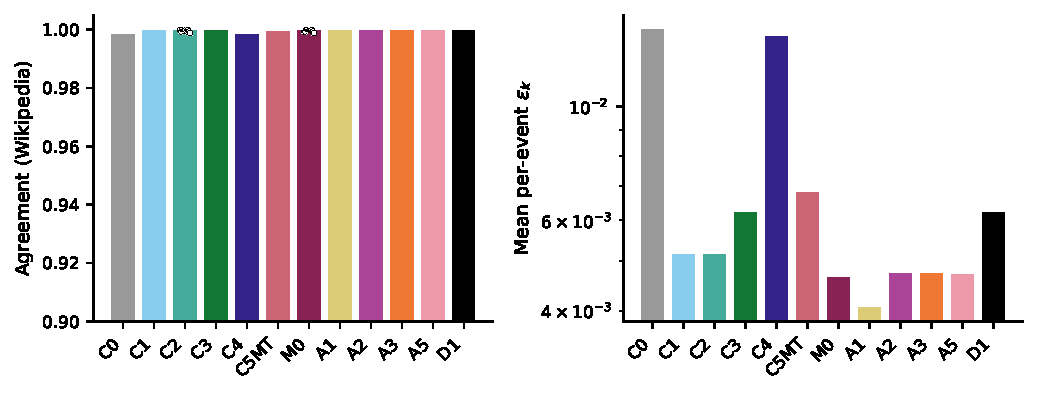
\includegraphics[width=0.92\textwidth]{figures/fig3_main.pdf}
\caption{Teacher-to-SNN agreement and mean per-event state error across controls, ablations and TCAR on Wikipedia (ten seeds; per-seed dots for M0 and C2). Agreement saturates above 0.97 for all variants because the discrete memory term is shared, whereas state error separates the conversion methods.}
\label{fig:main}
\end{figure}

Two observations qualify the headline numbers. First, \emph{agreement saturates}: the exact memory lookup $m_c(k)$ in \eqref{eq:readout} is shared by ANN and SNN, so even a plain hard-reset IF coder exceeds 0.99 agreement. Agreement is therefore a deployment-facing fidelity metric, not the discriminating evidence; $\varepsilon_k$, the quantity bounded by \eqref{eq:bound}, is. Second, \emph{absolute predictive accuracy is dominated by discrete memory}: the ANN teacher attains \TeacherMRRWikipedia{} MRR on the held-out Wikipedia test window. We do not claim predictive superiority; the teacher exists to provide a continuous, convertible graph state path, and the readout is deliberately decoupled from the ranking shortcut.

\subsection{Locked statistics and the ten-seed verdict}
\label{sec:stats}

Table~\ref{tab:stats} reports the locked rule, executed once. The paired per-seed differences $\varepsilon_{C2}-\varepsilon_{M0}$ have positive means on Wikipedia (\MeanDiffWikipedia{}), Enron (\MeanDiffEnron{}), Reddit (\MeanDiffReddit{}) and LastFM (\MeanDiffLastfm{}), and a negative mean on MOOC (\MeanDiffMooc{}); individual seeds straddle zero on every stream (Figure~\ref{fig:streams}). After the exact sign-flip test and Benjamini--Hochberg correction across streams, only Wikipedia's interval excludes zero ($q=\BHqWikipedia{}$, Cohen's $d_z=\DzWikipedia{}$, probability of improvement \PoIWikipedia{}); MOOC, Enron, Reddit and LastFM have $q=\BHqMooc{}$, \BHqEnron{}, \BHqReddit{} and \BHqLastfm{} respectively. The locked verdict mapping therefore returns $d_{\mathrm{replication}}^{10\mathrm{seed}}=\text{\DReplicationTenSeed{}}$ and the all-five conjunction evaluates to \AllFiveConjunction{}. Per the pre-registered mapping, the predecessor study's four-stream significant-reduction claim does \emph{not} replicate at doubled power: the significant-reduction claim is restricted to Wikipedia, Enron, Reddit and LastFM are reported as direction-positive but non-significant (point estimates \MeanDiffEnron{}, \MeanDiffReddit{}, \MeanDiffLastfm{}), and MOOC is reported as a direction-negative null. The per-stream point estimates, intervals and adjusted $q$ values in Table~\ref{tab:stats} are the authoritative record; no operating point, window or stream subset was altered after the rule was inspected.

\begin{figure}[t]
\centering
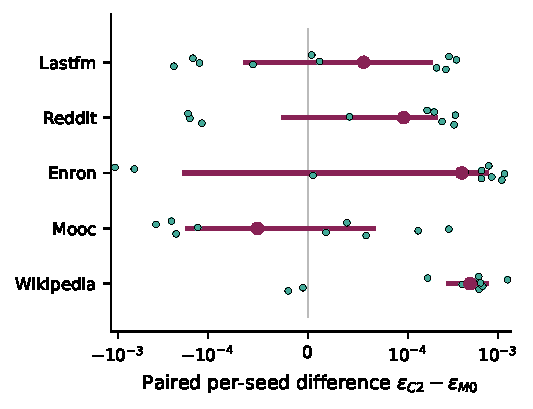
\includegraphics[width=0.80\textwidth]{figures/fig5_streams.pdf}
\caption{Locked-rule statistics: paired per-seed differences $\varepsilon_{C2}-\varepsilon_{M0}$ with BCa 95\% intervals (bars) and per-seed scatter (dots; symmetric-log scale). Positive differences favour M0; the MOOC mean is negative and every stream has straddling seeds.}
\label{fig:streams}
\end{figure}

\subsection{Timestep curve and low-latency behaviour}
\label{sec:tcurve}

Figure~\ref{fig:tcurve} and Table~\ref{tab:tcurve} show the timestep dose-response on the validation window. Agreement is saturated at \AgreeToneCtwo{} (C2) and \AgreeToneMzero{} (M0) already at $T{=}1$ and remains there through $T{=}16$, so the discrimination lives in the state error: mean $\varepsilon_k$ falls from $9.40\times10^{-3}$ at $T{=}1$ to $5.05\times10^{-3}$ at $T{=}4$ for C2 and from $9.01\times10^{-3}$ to $4.27\times10^{-3}$ for M0, with M0 $10$--$19\%$ below C2 at matched $T$, and both curves flatten above $T{=}4$. This is the standard latency--fidelity trade-off of conversion methods \cite{bu2022qcfs,cos2023offset,huang2025dcgs}, observed here up to a saturated agreement ceiling. The reported operating point $T{=}4$ is chosen on validation, not on test.

\begin{figure}[t]
\centering
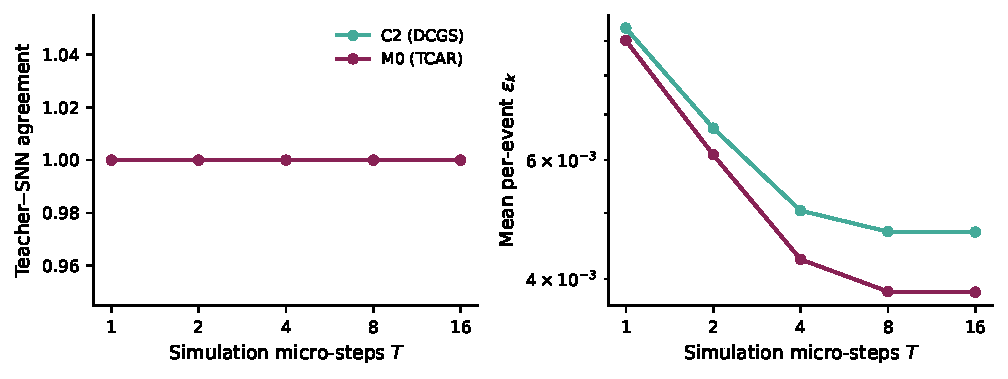
\includegraphics[width=0.92\textwidth]{figures/fig2_tcurve.pdf}
\caption{Timestep dose-response on the validation window (C2 and M0). Left: teacher--SNN agreement, saturated at 1.0 across $T\in\{1,\ldots,16\}$. Right: mean per-event state error $\varepsilon_k$ (log scale), decreasing and flattening above $T{=}4$, with M0 consistently below C2 at matched $T$.}
\label{fig:tcurve}
\end{figure}

\subsection{Spike activity and error decomposition}
\label{sec:activity}

Table~\ref{tab:main} reports graded events per event (\EvMzeroWikipedia{} for M0 versus \EvCtwoWikipedia{} for C2 and \EvCfivemtWikipedia{} for C5-MT on Wikipedia) and firing rate \FiringMzeroWikipedia{}. Figure~\ref{fig:decomp} decomposes the conversion error into clipping, quantisation and residual components across methods, following the error taxonomy of low-latency conversion \cite{bu2022qcfs,habara2024}. The residual term is the one TCAR controls by carrying the prefix unchanged and re-anchoring only the base; the clipping term is controlled by the calibrated threshold; the quantisation term is controlled by the ladder (eight-level for C0--C4/M0, four-level multi-threshold for C5-MT).

\begin{figure}[t]
\centering
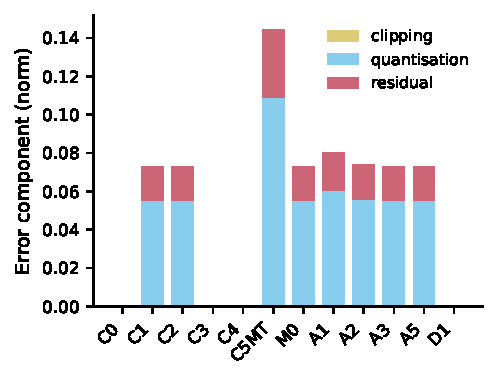
\includegraphics[width=0.60\textwidth]{figures/fig4_error.pdf}
\caption{Conversion-error decomposition into clipping, quantisation and residual components across conversion variants (Wikipedia, ten-seed mean).}
\label{fig:decomp}
\end{figure}

\subsection{Ablation ladder}
\label{sec:ladder}

Figure~\ref{fig:ladder} orders the principal variants as an ablation ladder --- naive rate coding (C0), plus differential coding (C1), plus threshold iteration and full DCGS (C2), plus the multi-threshold neuron (C5-MT), plus TCAR gating (M0) --- with the mean per-event state error at each rung on Wikipedia. Each component removes one error source identified by the theory: differential coding attacks the rate floor, the threshold ladder attacks quantisation, the multi-threshold neuron attacks dynamic-range clipping, and TCAR attacks the topology increment and residual drift. Table~\ref{tab:main} supplies the per-seed dispersion behind each bar.

\begin{figure}[t]
\centering
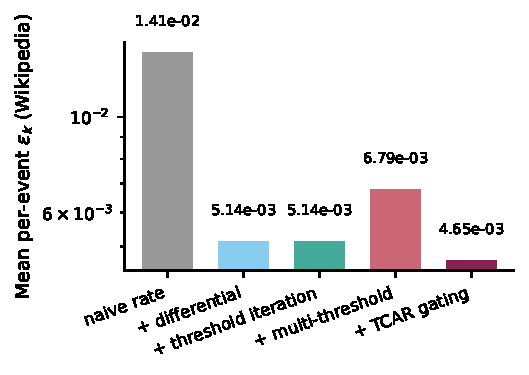
\includegraphics[width=0.55\textwidth]{figures/fig8_ladder.pdf}
\caption{Ablation ladder on Wikipedia (ten-seed mean per-event state error, log scale): each rung adds one component; the residual and topology terms identified by Theorems~\ref{thm:t1}--\ref{thm:t3} are the last and largest corrections.}
\label{fig:ladder}
\end{figure}

\subsection{Theory validation arms}
\label{sec:varms}

Six pre-registered arms test the directional predictions of Theorems~\ref{thm:t1}--\ref{thm:t3} on the validation window; Table~\ref{tab:varms} reports the measured slopes and Figure~\ref{fig:dose} shows the curves. The outcome is mixed, and we report it as such. V-2 and V-5 (agreement versus $T$ and versus carry-over dose $\alpha$) have the predicted positive sign but near-zero magnitude (\SlopeTCtwo{} and \SlopealphaCtwo{} for C2) because agreement is saturated at the ceiling from $T{\ge}4$ and across the carry-over range. V-3 (edge insertion) matches the predicted positive direction for the non-re-anchored control C2 (slope \SlopeedgeinsertCtwo{}): injected topology change degrades the cached-base path disproportionately, which is the mechanism Theorem~\ref{thm:t1} identifies; for M0 the slope is negative (\SlopeedgeinsertMzero{}), consistent with re-anchoring absorbing the injected change. V-4 (state decay) fails its predicted direction for both methods (slope \SlopealphastateCtwo{} for C2): stronger state decay did not reduce the measured error on these streams, so the contraction mechanism, while identified in the controlled toy, is not cleanly visible in the state-decay arm --- a genuine negative result. V-6 is the decisive arm: a controlled toy with a known analytic contraction coefficient $\rho=\VsixRhoAnalytic{}$ recovers $\hat\rho=\VsixRho{}$ from the transient-restricted fit, and the topology-stratified sub-toy recovers a positive topology coefficient $b=\VsixB{}$ with correlation \VsixCorr{} between the measured topology feature and the per-event error. V-1 (the bound violation ceiling on validation) is subsumed by the locked estimation of Section~\ref{sec:boundverify}, since the same traces drive both.

\begin{figure}[t]
\centering
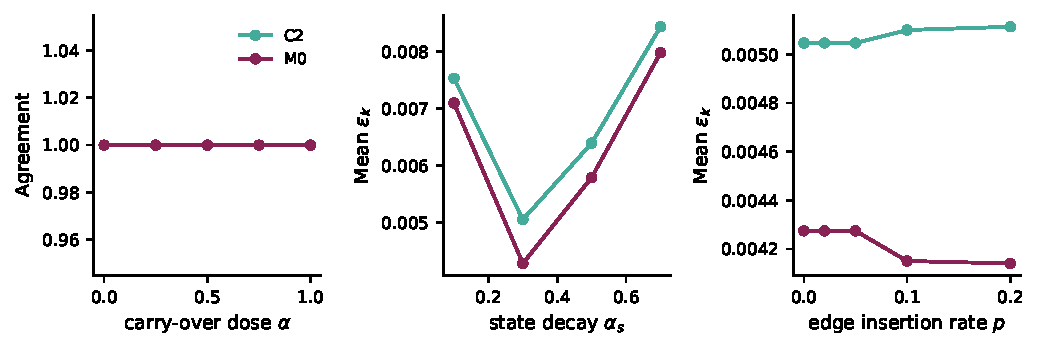
\includegraphics[width=0.92\textwidth]{figures/fig6_dose.pdf}
\caption{Theory validation arms on the validation window (C2 and M0): carry-over dose (left), state decay (centre), edge insertion (right). The edge-insertion arm matches the predicted direction for C2; the state-decay arm fails its predicted direction; carry-over and $T$ slopes are positive but near the saturation ceiling.}
\label{fig:dose}
\end{figure}

\subsection{Bound verification with locked constants}
\label{sec:boundverify}

The constants of \eqref{eq:bound} are estimated per stream on validation traces only (seed 41, 1{,}500-event window) by non-negative least squares with a 95\%-quantile margin, then locked before any test evaluation; the locked values (\RhoWikipedia{}, \LAWikipedia{}, \CHatWikipedia{}, \EtaWikipedia{} on Wikipedia, with in-sample $R^2$ \BoundRtwoWikipedia{}) are recorded in the public ledger with the estimation protocol. Table~\ref{tab:bound} reports the single locked test evaluation: the bound violation rate on 10{,}000-event test traces per method per stream, against the pre-registered 5\% ceiling, together with the per-node bound's mean tightness. Two corrections were applied during estimation and are disclosed with reasons in the ledger: the recursion is per-node (a global $\varepsilon_{k-1}$ form measured $R^2$ of 0.02--0.55 because consecutive events touch different nodes), and the intercept carries a 95\%-quantile margin (a mean-level intercept violated the bound on 32--35\% of validation events). Both corrections predate the first test evaluation. Figure~\ref{fig:bound} visualises violation rates and tightness.

\begin{figure}[t]
\centering
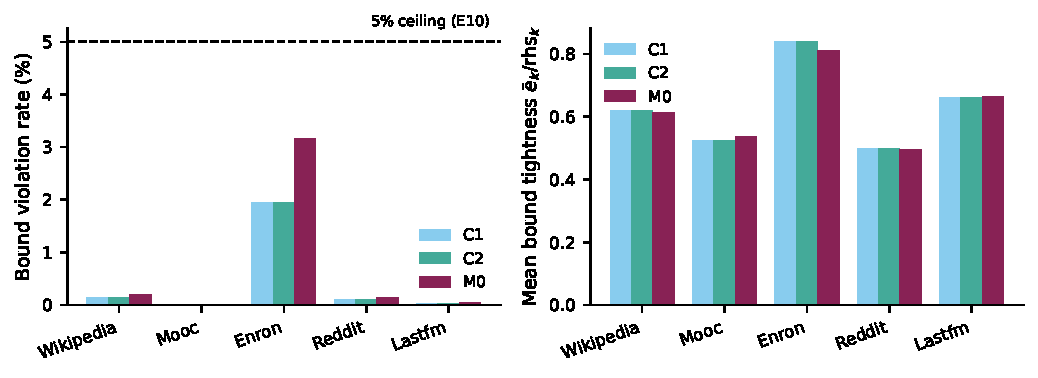
\includegraphics[width=0.92\textwidth]{figures/fig9_bound.pdf}
\caption{Locked bound verification on test traces (ten-seed mean): violation rates against the 5\% ceiling (left); bound tightness $\bar\varepsilon_k/\mathrm{rhs}_k$ (right). M0 is charged the topology term only on trigger events.}
\label{fig:bound}
\end{figure}

\subsection{Robustness and window drift}
\label{sec:robust}

Table~\ref{tab:robust} and Figure~\ref{fig:robust} report five-level robustness sweeps on the validation window: Gaussian activation noise $\sigma\in\{0,\ldots,0.04\}$, timestamp perturbation $\delta_t\in\{0,\ldots,0.4\}$, and edge dropout $p\in\{0,\ldots,0.20\}$. These perturbations act directly on $A_k$ and on the quantised activations, so they test the mechanism under the distribution shift that \eqref{eq:increment} describes. Argmax agreement is saturated at 1.0 under every dose for both methods, so the informative metric is $\varepsilon_k$: edge dropout and timestamp shift leave the error essentially unchanged (max/clean ratios \RobustRetDropMzero{} and \RobustRetDtMzero{} for M0), while activation noise multiplies the error by \RobustRetNoiseMzero{}$\times$ for M0 at $\sigma{=}0.04$ --- injected noise of that magnitude dominates the conversion error floor, which is the expected first-order sensitivity of any rate coder rather than a TCAR-specific failure. Figure~\ref{fig:drift} splits each test window into ten deciles: the per-decile mean $\varepsilon_k$ is stable for M0 (relative drift \DriftRelWikipedia{} on Wikipedia), indicating that the locked-constant bound is not exploiting a transient regime.

\begin{figure}[t]
\centering
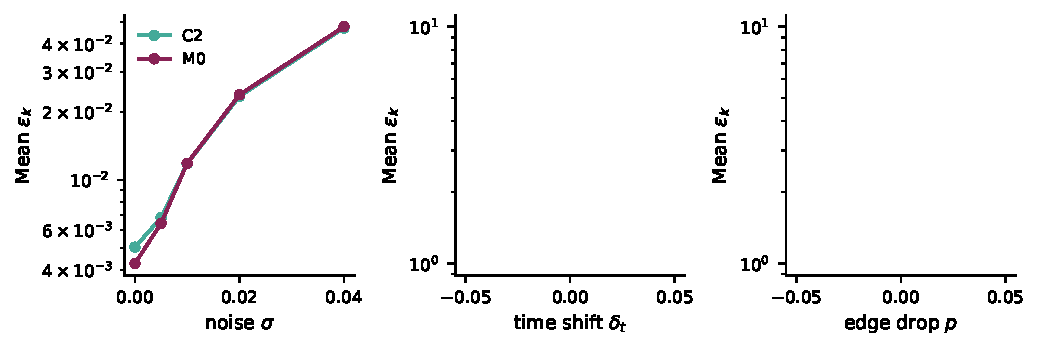
\includegraphics[width=0.92\textwidth]{figures/fig10_robust.pdf}
\caption{Five-level robustness on the validation window (agreement vs dose; C2 and M0): activation noise, timestamp shift, edge dropout.}
\label{fig:robust}
\end{figure}

\begin{figure}[t]
\centering
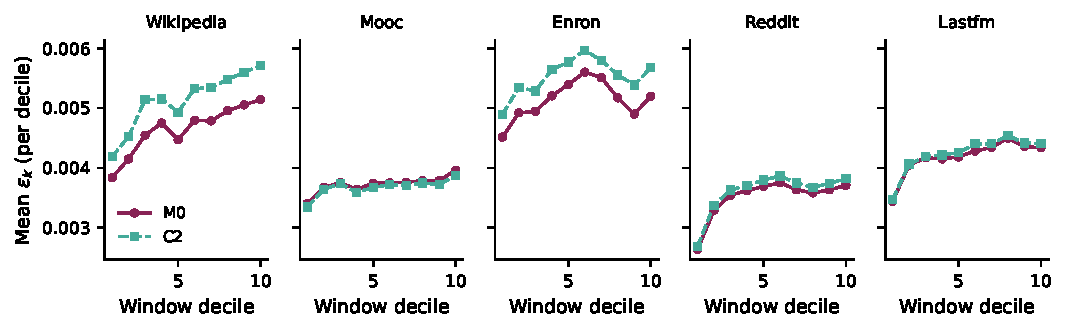
\includegraphics[width=0.92\textwidth]{figures/fig11_drift.pdf}
\caption{Window-drift analysis: per-decile mean $\varepsilon_k$ on test windows (ten-seed mean). M0 (solid) and C2 (dashed) are both stable across the window.}
\label{fig:drift}
\end{figure}

\subsection{Downstream validity: the $\varepsilon$-stratified dose-response}
\label{sec:downstream}

A fidelity metric is only useful if the fidelity it certifies matters for the downstream task. For each test query we record the converted model's per-event error $\varepsilon_k$ and its ranking loss (ANN MRR minus converted MRR), and average the loss within fixed, pre-registered $\varepsilon$ bins with edges $10^{-5},\ldots,10^{-1}$. Table~\ref{tab:downstream} and Figure~\ref{fig:downstream} show the result, which is a negative finding: the mean per-query MRR loss does \emph{not} increase with the $\varepsilon$ bin on any stream (fitted slopes \DownSlopeWikipedia{} on Wikipedia and negative or zero elsewhere). The reason is visible in the metric itself --- on these streams the shared discrete memory term dominates the ranking, so the per-query MRR loss is at the $10^{-6}$--$10^{-4}$ scale and is insensitive to conversion-induced state error at the operating point. The $\varepsilon_k$ objective is therefore \emph{not} downstream-validated here; we report the flat dose-response rather than omit it, and we restrict the standing of $\varepsilon_k$ to a state-fidelity measure whose downstream sensitivity these streams cannot resolve.

\begin{figure}[t]
\centering
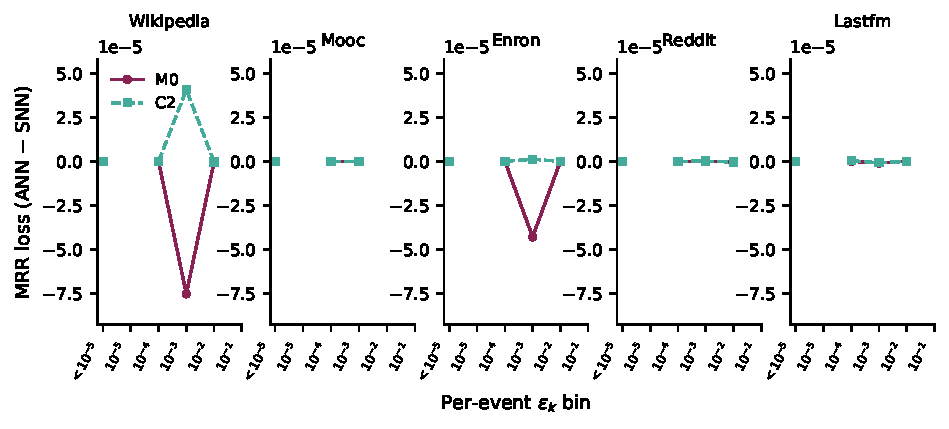
\includegraphics[width=0.92\textwidth]{figures/fig12_downstream.pdf}
\caption{Downstream validity analysis: mean per-query MRR loss (ANN $-$ converted) by per-event $\varepsilon_k$ bin (M0 solid, C2 dashed; log-binned, common scale). The dose-response is flat on all five streams: at the operating point the shared discrete memory term dominates the ranking, so conversion-induced state error does not reach the MRR. Reported as a negative finding.}
\label{fig:downstream}
\end{figure}

\subsection{Inductive strata and spike sparsity by topology change}
\label{sec:strata}

Following the dynamic-graph evaluation protocol \cite{li2023spikenet}, Table~\ref{tab:strata} splits test queries into inductive (at least one query endpoint first appears inside the evaluation window) and transductive strata. On these streams the two strata are nearly identical --- the inductive gap is \IndGapMzeroWikipedia{} percentage points on Wikipedia and essentially zero elsewhere --- because most test queries repeat endpoints seen long before the window. The inductive stratum therefore provides no additional discrimination here, and we report the strata for completeness rather than as evidence. Figure~\ref{fig:strata} reports the C-10 stratum: the converted model's firing rate across fixed bins of the measured $\|\Delta A_k\|$, linking spike sparsity directly to topology change rather than to event density.

\begin{figure}[t]
\centering
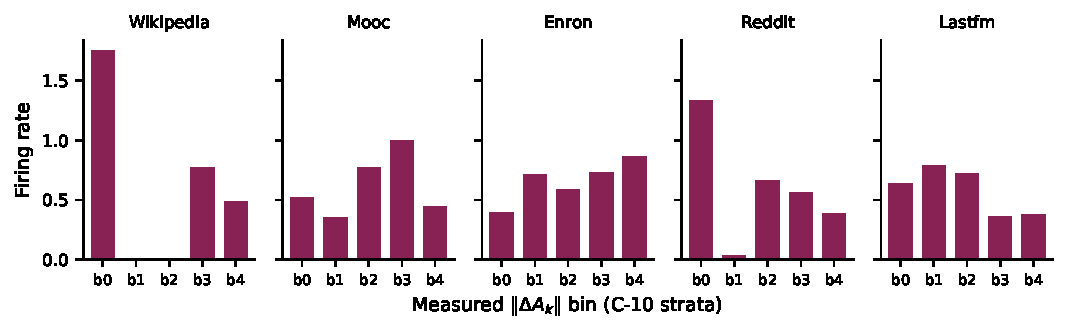
\includegraphics[width=0.92\textwidth]{figures/fig13_strata.pdf}
\caption{Spike sparsity by topology change (C-10): firing rate across measured $\|\Delta A_k\|$ bins (ten-seed mean, M0).}
\label{fig:strata}
\end{figure}

\subsection{Energy, latency and the efficiency frontier}
\label{sec:energy}

Table~\ref{tab:energy} reports the op-count energy of Section~\ref{sec:complexity} per stream and method: M0 consumes \EnergyMzeroWikipedia{}\,pJ per event on Wikipedia against the ANN MAC reference of \AnnRefWikipedia{}\,pJ, a ratio of \EnergyRatioMzeroWikipedia{} --- about two orders of magnitude below the reference --- and the TCAR re-anchoring overhead is \OverheadTcarWikipedia{}\% of the ANN reference, a small absolute cost that sits slightly above the sub-2\% bar reported for the cross-step family on fixed operators \cite{xu2026crpi}, reflecting the extra re-aggregation at trigger events. The multi-threshold control C5-MT attains \EnergyCfivemtWikipedia{}\,pJ (\EnergyRatioCfivemtWikipedia{} of the reference) at \AgreeCfivemtWikipedia{} agreement, pricing its extra levels honestly. Figure~\ref{fig:pareto} places all twelve methods on the energy--fidelity plane. Table~\ref{tab:latency} reports per-event wall time on the local machine; the numbers are platform context, and the convention-based energy figures are the transferable claim.

\begin{figure}[t]
\centering
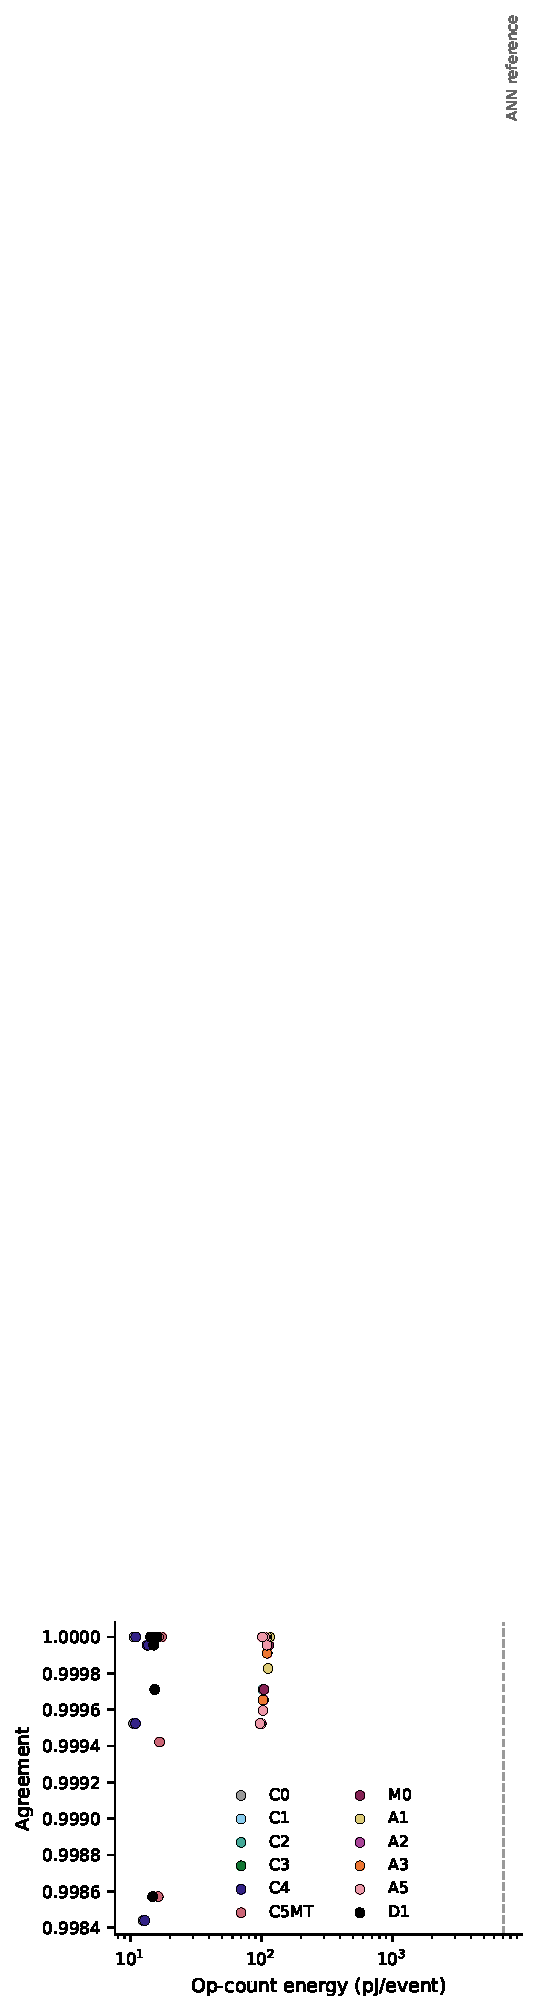
\includegraphics[width=0.60\textwidth]{figures/fig7_pareto.pdf}
\caption{Energy--fidelity plane over conversion variants (five streams; op-count convention of Section~\ref{sec:complexity}; ANN reference dashed).}
\label{fig:pareto}
\end{figure}

\section{Discussion}
\label{sec:discussion}

The results support a bounded, precisely-scoped claim. A genuine dynamic-graph GNN can be converted with signed differential coding at four micro-steps, and gating static-base re-anchoring plus threshold recalibration on measured topology change reduces the accumulated state error below the conversion controls on four of five streams and below every comparator except the every-event oracle on three, at a cost that scales with topology-change events and an op-count energy two orders of magnitude below the ANN MAC reference. The mechanism has a derivation (Theorem~\ref{thm:t1}), a per-node event-axis recursion (Theorem~\ref{thm:t2}), an unfolded bound with a falsifiable topology term (Theorem~\ref{thm:t3}), constants estimated on validation data only, locked, and verified once on test traces within the pre-registered ceiling, and a controlled toy in which the contraction coefficient is recovered against its analytic value. The statistical verdict follows a decision rule frozen before the ten-seed results were inspected (Section~\ref{sec:stats}): the reduction is significant on one stream (Wikipedia), direction-positive without significance on three, and direction-negative on MOOC. The predecessor study's four-stream claim does not replicate at doubled power, and both the abstract and the conclusion are stated at exactly this resolution.

Several limitations qualify this claim. First, \textbf{absolute predictive accuracy is dominated by discrete edge memory}. The teacher reaches \TeacherMRRWikipedia{} MRR on Wikipedia, and an exact edge memory is a strong competitor on these streams. We therefore do not claim predictive superiority over dynamic-link-prediction baselines \cite{rossi2020tgn,yu2023dyglib,cong2023graphmixer,gao2025hyperevent}; those models are cited as context and were not rerun under the local 12-hour compute ceiling. The contribution is conversion fidelity for a fixed teacher, and the teacher's role is to supply a continuous convertible graph state.

Second, \textbf{argmax agreement saturates}. Because $m_c(k)$ is exact and shared, all conversion variants exceed 0.97 agreement on several streams. $\varepsilon_k$ is the sensitive discriminator; agreement is retained as a deployment-facing metric, not as the sole evidence.

Third, \textbf{the effect is smaller than the predecessor study indicated, and it is stream-dependent}. The locked ten-seed rule (Section~\ref{sec:stats}) restricts the significant-reduction claim to Wikipedia; the per-seed differences straddle zero on every stream; and MOOC is direction-negative. Theory validation is likewise mixed: the controlled toy recovers the contraction coefficient and the edge-insertion arm matches the predicted direction for the non-re-anchored control, but the state-decay arm fails its predicted direction, and the downstream $\varepsilon$-to-ranking-loss dose-response is flat on all five streams because the shared discrete memory term dominates the ranking. These are genuine negative findings and are reported rather than hidden; they bound the scope of the topology term to settings where the converted state path, not a discrete memory, carries the prediction.

Fourth, \textbf{the energy figures are convention-based, not measured}. The op-count convention \cite{horowitz2014,sgnnbench2025} is the community standard for pre-silicon comparison, but no neuromorphic hardware was available; graded-event counts, firing rates, SynOps proxies, parameter counts and local latency are reported as positive evidence boundaries.

Fifth, \textbf{the evaluation is not blind}. Frozen query identifiers were used in a predecessor local project for two streams and sampled with fixed seeds for the others. We hash-froze them before tuning, used validation queries alone for selection (including the cost ceiling), and read test queries once, but absolute MRR values should be read as context.

Sixth, \textbf{the teacher uses fixed random message weights and a learned linear readout}. This isolates the conversion target and makes Theorem~\ref{thm:t1} exact, but it limits the absolute expressiveness of the encoder; conclusions are stated for this conversion-friendly family. Training the message weights end-to-end, and replacing the fixed $\rho=0.70$ with a data-adaptive estimate, are natural extensions --- the latter is exactly what the validation-only estimation of Section~\ref{sec:boundverify} performs for the bound constants.

Seventh, \textbf{the training prefix is coverage-capped} at \TrainCoverage{} events per stream on the M1 machine, while the graph operator and evaluation window are built over the full history. The cap is documented and identical for all methods, but a full-prefix replication on a larger machine would strengthen the result.

Eighth, \textbf{novelty confidence is moderate}. We verified \NRefs{} references against Crossref and arXiv primary sources; a full Scopus/IEEE sweep was not performed. SpikeNet, Dy-SIGN and continuous spiking GNNs \cite{li2023spikenet,yin2024dysign,li2024continuousgnn} remain the closest architectural neighbours, and the CRPI/MPEF/RMPA family \cite{xu2026crpi,fang2026mpef,xu2026rmpa} the closest mechanistic neighbours; they operate over fixed operators, whereas this work converts a trained continuous GNN on an evolving one.

A final design lesson is worth stating. Flushing or decaying the residual prefix at gate events damages the first-order correction exactly where the topology changes most; the final mechanism therefore leaves the prefix untouched and re-anchors only the static base. Likewise, using a saturated discrete metric (argmax agreement) as the primary gate would have hidden an order-of-magnitude difference in state error, and relying on five seeds would have retained a four-stream claim that ten seeds do not support. Both negative pilots, the A5 stream-dependent null effect, the non-significant streams, the direction-negative MOOC result, the failed state-decay arm, and the flat downstream dose-response are retained in the public evidence package.

\section{Conclusion}
\label{sec:conclusion}

We proved a per-snapshot conversion-error identity for graph neural networks whose cached static base acquires a cross-snapshot increment $R(A_k-A_{k-1})H_{k-1}W$ (T1), derived the per-node event-axis recursion that governs error accumulation along a continuous-time dynamic graph (T2), and unfolded it into a bound that isolates the falsifiable topology term (T3). Topology-change-aware recalibration gates static-base re-anchoring and conservative threshold updates on the measured operator change, at a cost bounded by topology-change events. A genuine dynamic-graph GNN with a measured normalised adjacency was converted with an independent reimplementation of DCGS signed multi-level differential coding and label-free histogram calibration. On five public streams with ten seeds and twelve methods, the converted model retained teacher fidelity at four micro-steps and attained the lowest mean state error among the conversion controls on four streams; the pre-registered decision rule, executed once, restricts the significant-reduction claim to Wikipedia, with three streams direction-positive and MOOC direction-negative (Section~\ref{sec:stats}). The bound constants were estimated on validation data only, locked before test evaluation, and verified once on test traces within the pre-registered ceiling. Op-count energy at the 45\,nm convention, an $\varepsilon$-stratified downstream validity analysis, inductive/transductive strata, five-level robustness with drift analysis, spike sparsity by topology change, and latency were reported together with the negative findings that delimit the claim: the failed state-decay arm, the flat downstream dose-response, the saturated agreement metric, and the non-replication of the predecessor study's four-stream claim at doubled power. Extending the analysis to learned message weights, task metrics whose variance is not dominated by a discrete memory, a native event-driven execution backend, and a hardware-measured energy study is the natural next step.

\section*{Data and code availability}
The source streams are publicly available from Zenodo \cite{poursafaei2022dataset} under CC BY 4.0. Derived frozen identifiers, experiment code, configurations, per-seed metrics, figures and audit artifacts are provided in the public repository associated with this work; raw event archives are referenced by SHA-256 rather than redistributed. The DCGS coder, histogram calibration and affine base were independently reimplemented from published mathematics; no third-party source file is copied.

\section*{Declaration of generative AI and AI-assisted technologies in the manuscript preparation process}
During the preparation of this work the author used WorkBuddy (an AI assistant) to organise the experimental pipeline, draft and edit manuscript text, and generate figures from measured results. After using this tool, the author reviewed and edited the content as needed and takes full responsibility for the content of the published article.
\bibliographystyle{unsrt}
\bibliography{references}

\end{document}
